% This is samplepaper.tex, a sample chapter demonstrating the
% LLNCS macro package for Springer Computer Science proceedings;
% Version 2.20 of 2017/10/04
%
\documentclass[sigplan,review,screen]{acmart}

% Generic definitions
% ===================

% Fix bad defaults
% ----------------
 
% We prefer varphi over phi.
\renewcommand{\phi} {\varphi}
% By subset we normally mean non-strict subset.
\renewcommand{\subset}  {\subseteq}


% logic operators
% ---------------

\newcommand {\lAnd} {\bigwedge}
\newcommand {\lOr} {\bigvee}
\newcommand {\limplies}{\rightarrow}
\newcommand {\liff}{\leftrightarrow}

\newcommand {\free}[1] {\mathsf{free}(#1)}
\newcommand {\fnot}[1] {\mathsf{not}(#1)}

% set operators
% -------------

\newcommand {\Intersection}  {\bigcap}
\newcommand {\Union}         {\bigcup}
\newcommand {\intersection}  {\cap}
\newcommand {\union}         {\mathrel{\cup}}
\newcommand {\disjointunion} {\mathrel{\sqcup}}

\newcommand {\powerset} {\mathcal P}
\newcommand {\N} {\mathbb{N}}

% Model theory
% ------------
 
\newcommand {\proves}{\vdash}
\newcommand {\satisfies}{\models}

% Matching Logic
% --------------
 
\newcommand {\Var}      {\mathsf{Var}}
\newcommand {\EVar}     {\mathsf{EVar}}
\newcommand {\SVar}     {\mathsf{SVar}}
\newcommand{\evaluation}[1]{\left| {#1} \right|}

% K
% -

\newcommand {\K}  {$\mathbb{K}$}

% Environments
% ------------

\usepackage{amsthm}
\newtheorem{theorem}                 {Theorem} [section]
\newtheorem{proposition}  [theorem]  {Proposition}
\newtheorem{lemma}        [theorem]  {Lemma}
\theoremstyle{definition}
\newtheorem{definition}   [theorem]  {Definition}
\newtheorem{remark}       [theorem]  {Remark}
\newtheorem{example}      [theorem]  {Example}

% Tables and figures share a counter
% ----------------------------------
\makeatletter 
\let\c@table\c@figure
\makeatother


% To do notes
% -----------

\usepackage{soul}
\newcommand {\todo}[1] {\hl{TODO: #1}}

% Paper Specific
% ==============
 
\usepackage{diagbox}

% Fragment Definitions
% --------------------

\usepackage{tikz}
\usetikzlibrary{shapes.misc, positioning}
\newcommand*\fragment[1]{
  \tikz[baseline=(char.base)]{\node[draw,rectangle,rounded corners=2pt,inner sep=2pt,fill=black,text=white] (char){\phantom{\rlap{fgq}}$\mathsf{#1}$};}
}
\newcommand{\structure}      { \fragment{structure} }
\newcommand{\logic}          { \fragment{logic} }
\newcommand{\quantification} { \fragment{quantification} }
\newcommand{\fixedpoint}     { \fragment{fixedpoint} }

% Signatures
\newcommand{\umeasure}{\mathsf{Measure}^\mu}
\newcommand{\vmeasure}{\mathsf{Measure}^\nu}


% Status Quo table
% ----------------

\usepackage{pifont}
\usepackage{newunicodechar}
\newunicodechar{✓}{\ding{51}}
\newunicodechar{✗}{\ding{55}}
\newunicodechar{⍻}{\ding{55}}
\newcommand{\cmark}{{\ding{51}}}%
\newcommand{\qmark}{{\textbf ?}}%
\newcommand{\xmark}{{  \ding{55}}}%
\newcommand{\cxmark} {{\ding{51}}\textsuperscript{\kern-0.47em\tiny\ding{55}}}
\newcommand{\fin}{$_\mathrm{fin}$}
\renewcommand{\inf}{$_\mathrm{inf}$}

% Definition list, Tableau & Sequents
% -----------------------------------
 
\newcommand{\deflist}{\mathcal D}
\newcommand{\mkDeflist}[1]{\mathsf{deflist}(#1)}
\newcommand{\combineDefList}{\circ}

\newcommand{\matches}[2]{\mathsf{matches}(#1,\allowbreak #2)}
\newcommand{\sequent}[1]{\left\langle #1 \right\rangle}
\newcommand{\Sequent}{\mathsf{Sequent}}
\newcommand{\unsat}{\mathsf{unsat}}
\newcommand{\sat}{\mathsf{sat}}
\newcommand{\valid}{\mathsf{valid}}
\newcommand{\Basic}{\mathcal{B}}
\newcommand{\Universals}{\mathcal{U}}
\newcommand{\Elements}{\mathcal{E}}

\newcommand{\name}[1]{\text{(#1)}}
\newcommand{\dapp}   {$\overline{\mbox{app}}$}

\newcommand{\pruleun} [2]{\displaystyle\frac{#1}{#2}}
\newcommand{\prulebin}[3]{\displaystyle\frac{#1}{#2\qquad#3}}
%\newcommand{\prulebin}[3]{$$\frac{#1}{#2\quad#3}$$}
\newcommand{\prftree}[3][YYY]{XXX \frac{#1}{#2\quad#3}}

\newcommand{\satruleun}[2]      {{\pruleun{#1}{#2}}}
\newcommand{\satrulebin}[3]     {{\prulebin{#1}{#2}{#3}}}
\newcommand{\unsatruleun}[2]    {{\pruleun{#1}{#2}}}
\newcommand{\unsatrulebin}[3]   {{\prulebin{#1}{#2}{#3}}}

\newcommand{\inst}{\mathsf{inst}}

\newcommand{\vruleun}[2]{\frac{#2}{#1}}
\newcommand{\vrulebin}[3]{\frac{#2\quad#3}{#1}}

% QF Tableau
% ----------

\newcommand{\wit}{\mathit{wit}}
\newcommand{\Wit}{\mathit{Wit}}
\newcommand{\SSS}{\mathcal{S}}
\newcommand{\SSSmod}{\mathcal{S}_\mathrm{mod}}
\newcommand{\appa}{\prule{choose-app}}
\newcommand{\appb}{\prule{choose-wit}}
\newcommand{\appc}{\prule{app}}
\newcommand{\rt}{\mathit{root}}
\newcommand{\Nodes}{\mathsf{Nodes}}
\newcommand{\contr}[1]{[\!\rangle #1 \langle\!]}
\newcommand{\expan}[1]{\langle\!] #1 [\!\rangle}
\newcommand{\seq}{\mathit{seq}}
\newcommand{\prule}[1]{\textsc{(#1)}}
\newcommand{\Tr}{\mathit{Tr}}
\newcommand{\Pattern}{\textsf{Pattern}}
\newcommand{\wbar}{\overline}
\newcommand{\SigD}{\umeasure}
\newcommand{\SignD}{\mathsf{SignD}}
\newcommand{\DD}{\deflist}
\newcommand{\nDD}{\deflist^{\nu}}
\newcommand{\alphab}{{\bar\alpha}}

\newcommand{\pto}{\rightharpoonup}
\newcommand{\dom}{\mathrm{dom}}
\DeclareMathOperator*{\argmax}{arg\,max}
\DeclareMathOperator*{\argmin}{arg\,min}
\newcommand{\des}{\mathit{des}}
\newcommand{\Aut}{\mathcal{A}}

% Games
% -----

\newcommand {\dependson}{\prec^\phi}
\newcommand {\Pos}{\mathrm{Pos}}
\newcommand {\game} {\mathcal G^{\mathcal T}}
\newcommand {\PosT} {\Pos^{\mathcal T}}
\newcommand {\ET}   {E^{\mathcal T}}
\newcommand {\OmegaT}   {\Omega^{\mathcal T}}

% Miscelanious
% ============

\newcommand{\FF}{\mathcal{F}}
\newcommand{\PP}{\mathcal{P}}
\newcommand{\TT}{\mathcal{T}}

\newcommand{\size}[1] {\left\lVert #1\right\rVert}
\newcommand{\width}[1]{\mathrm{width}(#1)}

\newcommand {\where}[1]
            {{\footnotesize\quad\parbox[t]{0.3\textwidth}{where #1 }}}

\usepackage{multicol}

% End of LaTeX Prelude
% --------------------

\usepackage{graphicx}
\makeatletter
\def\maxwidth{\ifdim\Gin@nat@width>\linewidth\linewidth\else\Gin@nat@width\fi}
\def\maxheight{\ifdim\Gin@nat@height>\textheight\textheight\else\Gin@nat@height\fi}
\makeatother
% Scale images if necessary, so that they will not overflow the page
% margins by default, and it is still possible to overwrite the defaults
% using explicit options in \includegraphics[width, height, ...]{}
\setkeys{Gin}{width=\maxwidth,height=\maxheight,keepaspectratio}

\graphicspath{{figs/}}

\newcommand{\tightlist}{}

\begin{document}

\title{Decidable Fragments of Matching Logic}
\begin{abstract}
    Matching logic has been put forward as a "lingua franca"
    for verifying and reasoning about programs and programming languages.
    We propose three increasingly powerful decidable fragments of matching logic.
    The largest of these fragments, called the guarded fragment,
    allows both fixedpoints and a restricted form of quantification.
    It is intended to extend the automated prover for uniform reasoning across
    logics in a previously developed framework,
    by providing a robust basis for unfolding fixedpoints and simplification.
\end{abstract}

\maketitle
\emergencystretch 5em

\hypertarget{sec:introduction}{%
\section{Motivation}\label{sec:introduction}}

The recent proliferation of programming languages has brought into focus the
need for a carefully streamlined language infrastructure.
Computation, and therefore programming languages, have begun to pervade every
domain of our being, from our day-to-day lives in our pockets and our homes,
to financial instruments and quantum computing.
Each of these languages are tailored to their specific domain, and yet, rightfully,
users demand sophisticated tooling for optimized compilation, debugging, model
checking and program verification.
Implementing such tooling on a language-by-language basis is not just redundant,
but also cost-prohibitive.
Creating tooling that provides a depth in terms of quality and complexity,
while still covering this breadth of diversity of languages and their domains
requires that we systematically streamline these redundancies.

We envision an \emph{ideal language framework}, shown in Figure \ref{fig:ideal-framework},
where a language designer must only provide
a formal description of the syntax
and a formal semantics for their language,
from which language tooling may be automatically generated ``for free'' by the framework.

\begin{figure}
\hypertarget{fig:ideal-framework}{%
\centering
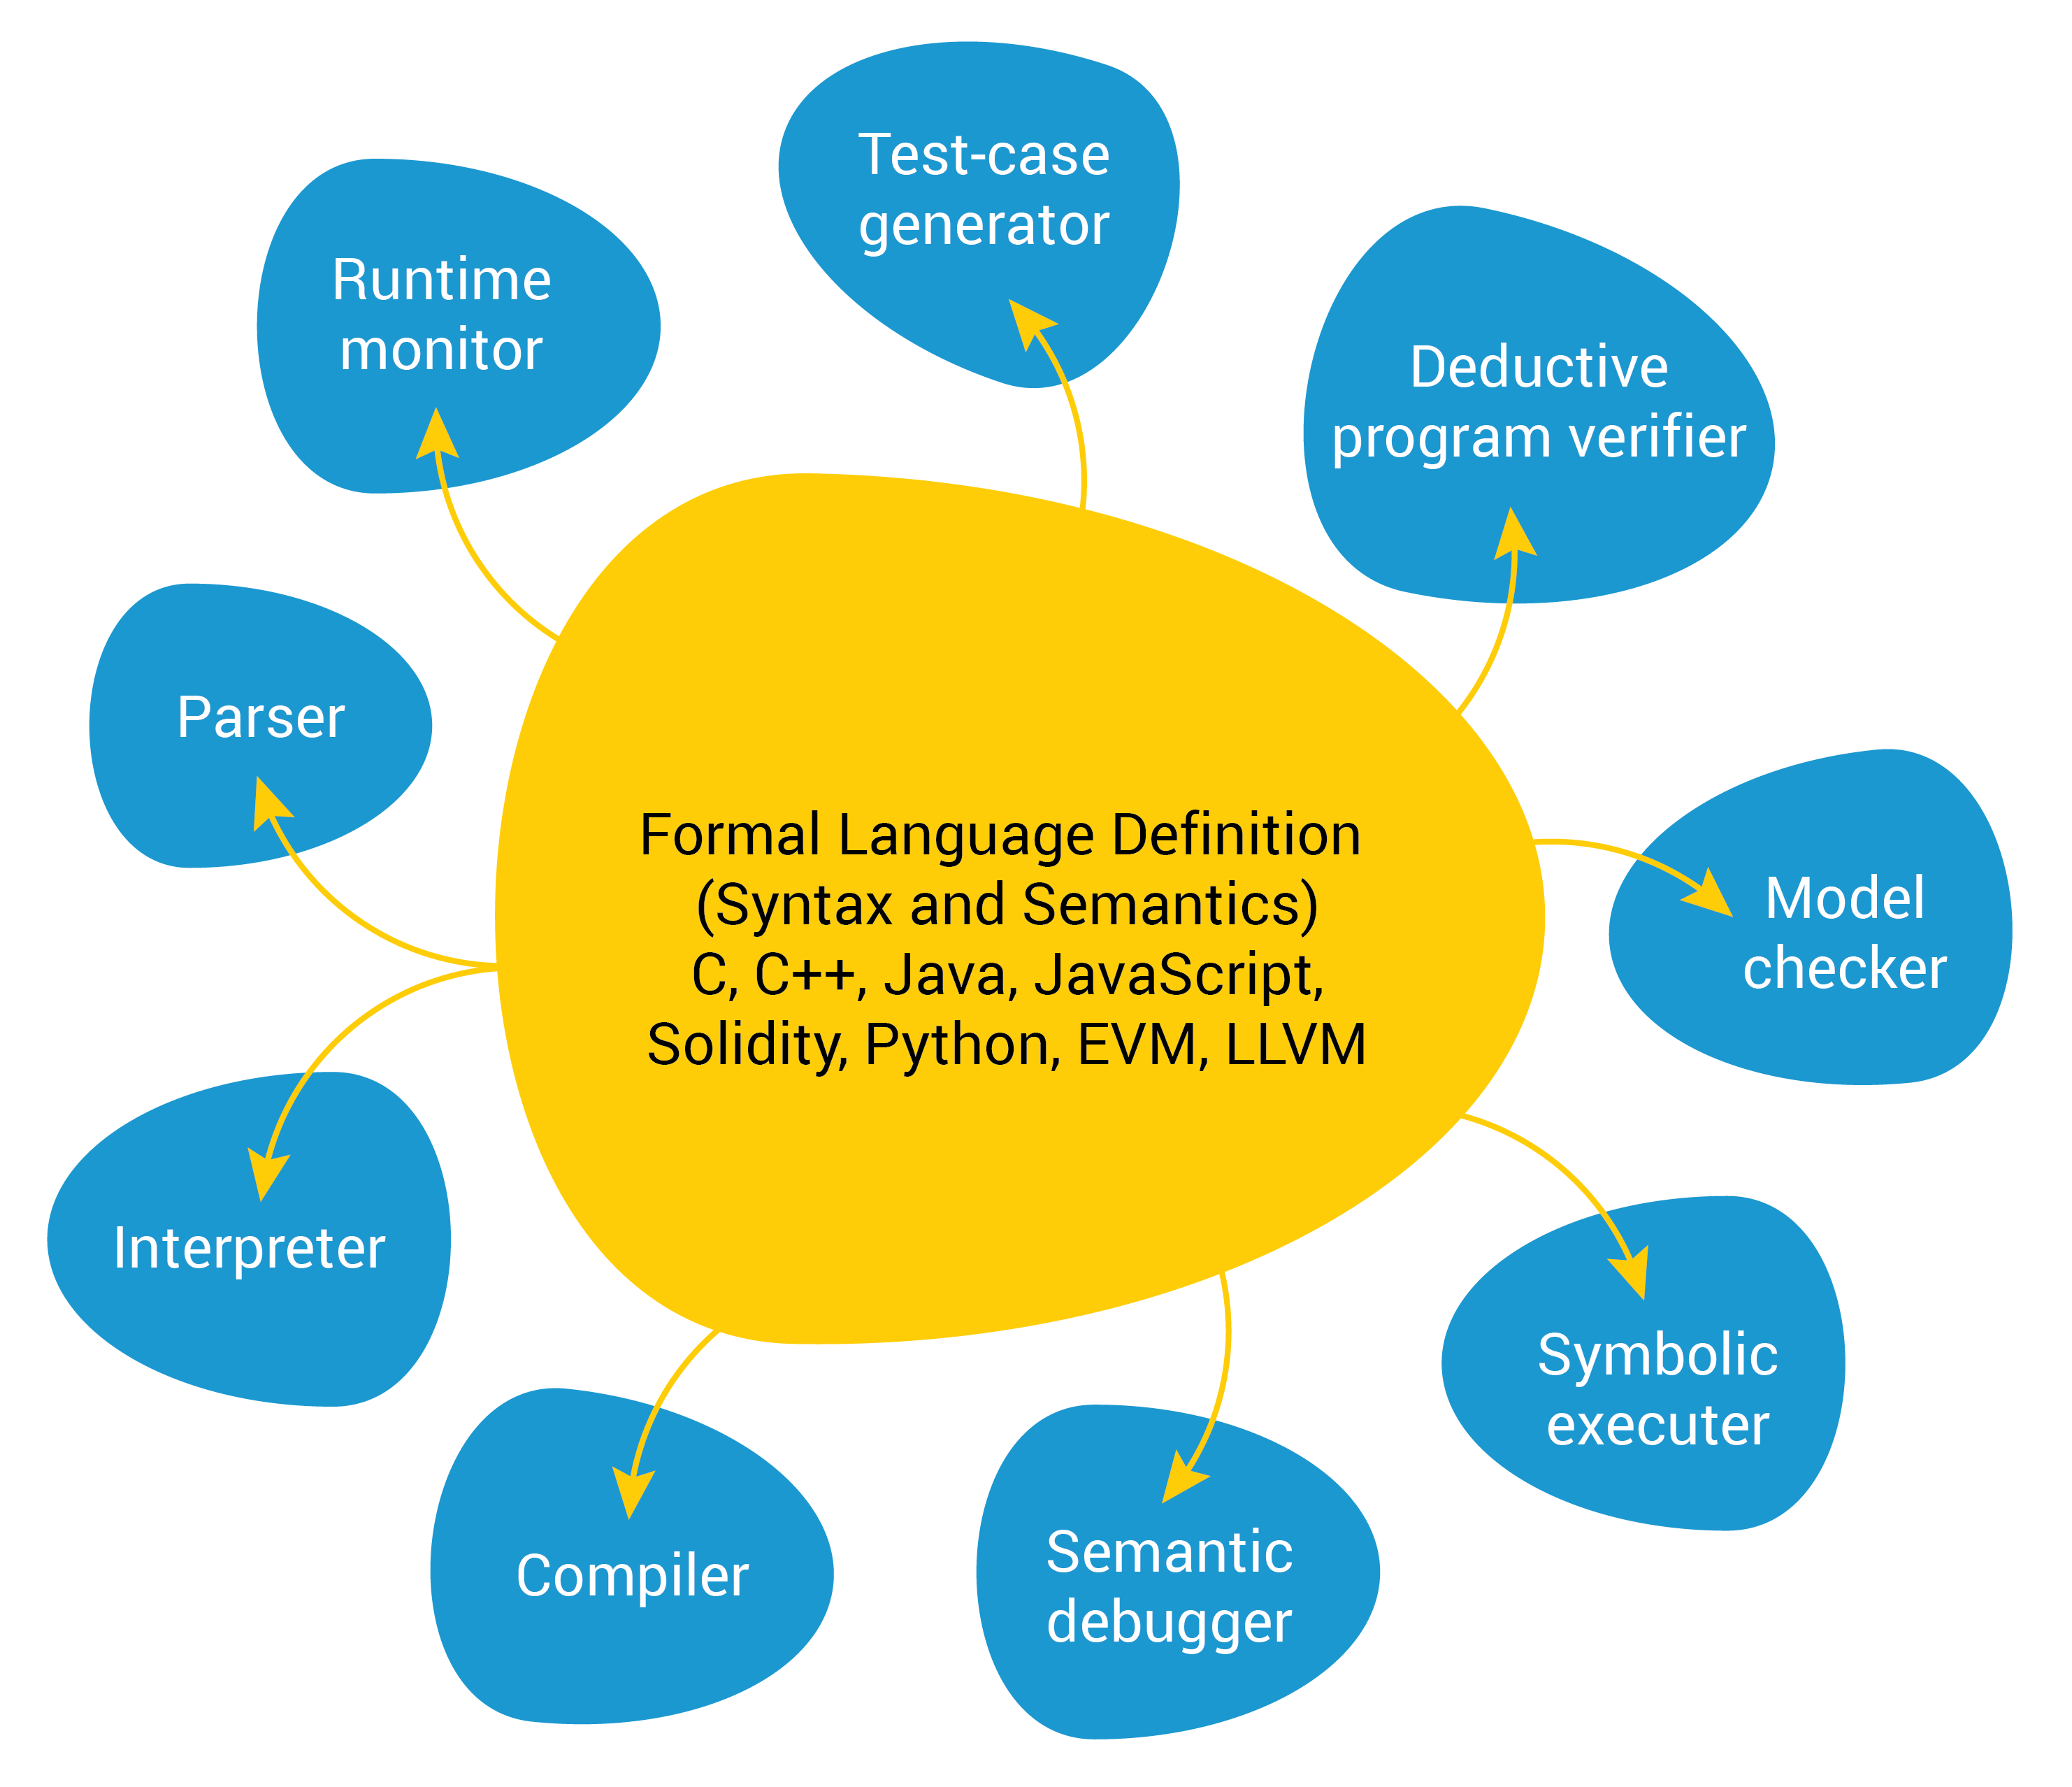
\includegraphics[width=0.45\textwidth,height=\textheight]{figs/ideal.png}
\caption{An ideal language framework: all language tools are generated from a formal language semantics.}\label{fig:ideal-framework}
}
\end{figure}

The \K{} framework (\url{https://kframework.org}) pursues this vision.
\K{} provides an intuitive meta-language with which language designers
may define the formal semantics of their programming language
as a transition system.
The framework uses this to generate
parsers, interpreters, deductive verifiers \cite{SPY+16,Ros17a},
program equivalence checkers \cite{kasampalis2021language}, among others.
This approach is no longer of purely academic interest---diverse and complex programming languages have been specified in \K{}
including \cite{c-semantics}, Java \cite{java-semantics}, JavaScript \cite{javascript-semantics},
EVM \cite{evm-semantics} and x86 assembly \cite{x86-semantics}.
The commercial success of verification tools built using this approach (e.g.~\url{https://runtimeverifcation.com}) show that these tools are practical, valuable
and in-demand.

In order to provide sound and powerful formal verification tools \K{} needs a firm logical foundation.
Without such a logical foundation the very meaning of what it means for a program to be ``verified'' or ``correct'' are in question.

Matching logic \cite{matchinglogiclmcs,matching-mu-logic,matching-logic-explained} provides this foundation.
As shown in Figure \ref{fig:ml-as-basis-for-k}, every \K{} semantic definition of a language \(L\) yields a corresponding matching logic theory \(\Gamma_L\),
and every language task, such as executing a program or verifying a property, conducted by \K{}
is characterized by checking the validity of a matching logic entailment,
\(\Gamma_L \vdash \phi_\mathit{task}\), where \(\phi_\mathit{task}\) is the formal specification of the task in matching logic.
These language tasks range from running a program in an interpreter
(i.e.~checking if there is a terminating execution trace for a program),
to proving reachability claims.
If these tools emit proof certificates, they may be checked with the matching logic proof checker \cite{chen-lin-trinh-rosu-2021-cav}.

\begin{figure}
\def\svgwidth{\columnwidth}
\newcommand{\kbox}[1]{
    \tikz[baseline=(char.base)]{\node[draw,rectangle,rounded corners=2pt,inner sep=2pt] (char){\phantom{\rlap{yL$._y$}}#1};}
}
\newcommand{\g}[1]{$\Gamma_\text{#1}$}
\input{figs/ml-as-basis-for-k.pdf_tex}
\caption{Matching Logic as the foundation for \K{}}
\label{fig:ml-as-basis-for-k}
\end{figure}

Matching logic provides this foundation by creating a unifying logic, or \emph{lingua franca}, for formal verification.
Constructs for building terms, first-order quantification, and fixedpoints,
allow capturing the many formalisms important to verification,
including linear temporal logic (LTL) \cite{ltl}, computation tree logic (CTL) \cite{ctl}, separation logic (SL) \cite{separation-logic}, and
reachability logic \cite{matchinglogiclmcs,matching-mu-logic},
as well as the language-semantics-as-a-theory produced by \K{}.
Together, these may be used to define the various language tasks described above.
It does all this while maintaining minimal \emph{representational distance}---because
it preserves and respects the original syntactic and semantic structures,
such as program ASTs, continuations, heaps and stacks, language semantics may be captured in a compact and modular way.
In fact, the embeddings of many logics are syntactically identical to the original logics.
This is in contrast to approaches that translate these to, say, first-order logic,
that introduce quantifiers and other clutter.

\K{}'s tools are best-effort checking for the validity of these entailments.
Currently, this is done through ad-hoc reasoning developed on an as-needed basis
and translation to SMT-LIB2 \cite{smtlib} for dispatch to the Z3 solver \cite{z3}.
This leads to quite a few deficiencies---limited support for induction,
users need to spell out many lemmas and simplifications,
caching and optimization are at the mercy of what Z3's incremental interface will accept.
\newline

\emph{Our grand vision is to develop a matching logic solver, systematically and methodically,
that unifies reasoning across embedded logics, and alleviates these problems.}
In \cite{towards-a-unified-framework}, the authors took the first steps in this
effort---they build the foundations for a unified proof framework that allows
fixedpoint reasoning across logics.
The authors developed a set of
high-level (relative to matching logic's own proof rules)
syntax-driven proof system, amenable to automation.
This approach was effective---the framework was evaluated against four logical
systems---first-order logic with fixedpoints, separation logic, reachability
logic, and linear temporal logic (LTL).

However, as admitted in \cite{towards-a-unified-framework} itself, it would be unreasonable
to hope that at such a nascent stage this framework would be able to compete with
state-of-the-art domain-specific provers and decision procedures.
We, however, believe that such a goal is possible and within reach in the near-term, but will
likely take several years of sustained effort.
Such an effort is worthwhile, because if successful could be transformative to the fields
of automated deduction and program verification.

In this work, we take aim at some shortcomings of this framework.
First, the core of the framework was based on an ad-hoc unfolding of fixedpoints.
The boundaries of where this procedure is complete, and when it would not terminate are not known.
To work around this, an arbitary bound on the number of unfoldings for fixedpoints.
Further, the procedure unnecessarily tried all possible interleavings of unfoldings
leading to poor performance when there were more than a few fixedpoints in the claim.
Second, the framework peformed poorly with arbitary claims, getting ``stuck'' when not in a specific normalized form.
Often the simplification procedures weren't powerful enough to re-normalize between applications of these strategies.
\todo{make sure we answer precisely how these are solved later in the paper.}

We propose that this heuristic be replaced with a decision procedure for a fragment of matching logic,
analogously to how DPLL \cite{dpll,dpllt}, a decision procedure for propositional fragment of first-order logic,
forms the core of many first-order SMT solvers \cite{z3,mathsat4,cvc4}.
Solvers for first-order logic are typically constructed around DPLL,
an algorithm for checking the satisfiability of propositional logic formulae.
A first-order formula is transformed into a propositional ``skeleton'' by replacing atoms with propositional variables.
The DPLL algorithm then produces solutions to this skeleton---truth assignments to each of the introduced propositional variables.
If any of these solutions are consistent with the atoms from the original formula,
then the entire first-order formula is satisfiable.

Unfortunately, DPLL cannot directly be used in the same way as the core for matching logic automated proving
because matching logic formulae (called ``patterns'') cannot be reduced to a propositional skeleton.
This is because matching logic patterns are interpreted as the set of elements
they match, unlike propositional variables which are two-valued (either true or false).
In fact, translation to first-order logic or other logics is not desired in general,
because the additional complexity, such as quantifiers,
thwarts the nice properties such as compactness and modularity gained by using matching logic.
In addition, since fixedpoint reasoning is an important aspect of program verification,
the core motivation for matching logic,
and it would be ideal if inductive reasoning is built into this core.
\newline

\emph{In this paper we propose three increasingly powerful decidable fragments of matching logic.}
Despite being redundant, presenting all three fragments allows us to incrementally introduce the techniques used
instead of forcing the reader to deal with the complexity all at once.

\begin{figure}
\def\columnwidth{\columnwidth}
\newcommand{\g}[1]{$\Gamma_\text{#1}$}
\input{figs/decidable-theories.pdf_tex}
\caption{Proposed decidable fragments of matching logic, and some decidable embedded logics they subsume.}
\end{figure}

The first and simplest fragment is called the \emph{modal fragment} and allows neither fixedpoints nor quantification.
To those familiar with modal logic, it may be thought of as a polyadic multimodal form of this logic.
We prove that this fragment is decidable by showing that it has the small-model
property---the size models for satisfiable are bound by a computable function of the size of the pattern.

The second fragment, the \emph{quantifier-free fragment}, extends this to allow
least- and greatest-fixedpoints, the modal \(\mu\)-calculus extension of modal logic.
This is proved decidable through an extension to the approach
first show in \cite{games-for-mu-calculus}.

The final fragment, called the \emph{guarded fragment},
allows both fixedpoints and a restricted form of quantification.
Again, this is proved decidable through an extension to the corresponding
decision procedure for guarded fixedpoint logic.
We introduce a resolution-like rule that plays the role of backtracking in DPLL.
It also removes the need to iterate over all possible interpretations
(as required by the algorithm presented by Grädel).
and gives us a tangible object, called a refutation, in case the pattern is unsatisfiable.
We may later work on a way of converting this to a formal proof.
We propose using the presented decision procedure for this fragment as a new
core for the proof framework in \cite{towards-a-unified-framework}.

\hypertarget{sec:ml-prelims}{%
\section{Matching Logic Preliminaries}\label{sec:ml-prelims}}

Matching logic was first proposed in \cite{matchinglogiclmcs} as a unifying logic
for specifying and reasoning about programming languages.
An important feature of matching logic is that it makes no distinction between terms and formula.
This flexibility makes many important concepts easily definable in matching logic,
and allows for awkwardness free encodings of various abstractions and logics possible.
For example,
LTL formulae have identical syntax to their embedding in matching logic,
and unification may be characterized by conjuncting two pattern built from constructors.

Matching logic formulae are called \emph{patterns}
and have a ``pattern matching'' semantics,
in the sense that each pattern represents the set of elements that ``match'' it.
For example, \(\mathsf{cons}(42, x)\) matches lists whose first element is \(42\),
while \(\mathsf{prime} \land \mathsf{even}\) matches the natural \(2\),
assuming correct axiomatizations for \(\mathsf{cons}\), \(\mathsf{prime}\), and \(\mathsf{even}\).

\hypertarget{matching-logic-syntax}{%
\subsection{Matching Logic Syntax}\label{matching-logic-syntax}}

For a set \(\EVar\) of \emph{element variables}, denoted \(x, y, z, \ldots\),
and a set \(\SVar\) of \emph{set variables}, denoted \(X, Y, Z, \ldots\), we define the syntax of matching logic below.

\begin{definition}[Matching logic signatures]A matching logic \emph{signature}, \(\Sigma\) is a set of symbols with an associated arity.
Symbols with an arity of zero are called \emph{constants}.\end{definition}

\begin{definition}[Patterns]Given a signature \(\Sigma\), a countable set of element variables \(\EVar\) and of set variables \(\SVar\),
a matching logic \emph{pattern} is built recursively using the following grammar:
\begin{align*}
\phi:=  \underbrace{\sigma(\phi_1, \dots, \phi_n)}      _\text{\structure{}}
  \mid  \underbrace{\phi_1 \land \phi_2 \mid \lnot \phi}_\text{\logic{}}
  \mid  \underbrace{x \mid \exists x \ldotp \phi}       _\text{\quantification}
  \mid  \underbrace{X \mid     \mu X \ldotp \phi}       _\text{\fixedpoint{}}
\end{align*}
where \(x \in \EVar\), \(X \in \SVar\) and \(\sigma \in \Sigma\) has arity \(n\), and \(X\) occurs only positively in \(\mu X\ldotp \phi\). That is, \(X\) may only occur under an even number of negations in \(\phi\).\end{definition}

We assume the standard notions for free variables, \(\alpha\)-equivalence, and capture-free substitution \(\phi[\psi/x]\)
and allow the usual syntactic sugar:
\begin{align*}
                       \top &\equiv \exists x \ldotp x &
                       \bot &\equiv \lnot \top \\
         \phi_1 \lor \phi_2 &\equiv \lnot(\lnot\phi_1 \land \lnot\phi_2) &
    \phi_1 \limplies \phi_2 &\equiv \lnot \phi_1 \lor \phi_2 \\
      \forall x \ldotp \phi &\equiv \lnot \exists x \ldotp \phi &
      \nu X \ldotp \phi &\equiv \lnot \mu X \ldotp \lnot \phi[\lnot X/X]
\end{align*}
\(\sigma(\phi_1, \dots, \phi_n)\) are called applications.
Nullary applications are called constants, are denoted by using \(\sigma\) instead of \(\sigma()\).

\hypertarget{sec:semantics-of-matching-logic}{%
\subsection{Semantics of Matching Logic}\label{sec:semantics-of-matching-logic}}

Unlike in FOL, matching logic patterns are interpreted as a set of elements in a model rather than a single element.
Intuitively, the interpretation is the set of elements that match a pattern.
For example, the constant \(\mathsf{even}\) might have as interpretation the set of all even naturals,
while \(\mathsf{greaterThan}(3)\) may be interpreted as all integers greater than \(3\).
Function symbols may be considered a special case of this, where when applied to an argument the interpretation is a singleton set.
Logical constructs are thought of as set operations over matched elements
-- for example, \(\phi \land \psi\) is interpreted as the intersection of elements matched by \(\phi\) and \(\psi\),
while \(\lnot \phi\) matches all elements \emph{not} matched by \(\phi\).
An existential \(\exists x \ldotp \phi(x)\) is interpreted as the union of all patterns matching \(\phi(x)\) for all valuations of \(x\).
\(\mu X \ldotp \phi(X)\) matches the \emph{least} set \(X\) such that \(X\) and \(\phi(X)\) match the same elements.
An important point to note here is that element variables have as evaluation exactly a single element,
whereas set variables may be interpreted as any subset of the carrier set.

\begin{definition}[\(\Sigma\)-models]Given a signature \(\Sigma\), a \(\Sigma\)-model is a tuple \((\mathbb M, \{ \sigma_M \}_{\sigma \in \Sigma} )\)
where \(\mathbb M\) is a set of elements called the carrier set,
and \(\sigma_M : M^n \to \powerset(M)\) is the interpretation of the symbol \(\sigma\) with arity \(n\) into the powerset of \(M\).\end{definition}

We use \(M\) to denote both the model \(M\), and it's carrier set, \(\mathbb M\).
We also tacitly use \(\sigma_M\) to denote the pointwise extension, \(\sigma_M : \powerset(M)^n \to \powerset(M)\),
defined as \(\sigma_M(A_1,\dots,A_n) \mapsto \Union_{a_i\in A_i} \sigma_M(a_1,\dots,a_n)\)
for all sets \(A_i \subseteq M\).

\begin{definition}[Semantics of matching logic]\label{def:semantics}Let \(\rho : \EVar{} \union \SVar{} \to \powerset(M)\) be a function such that \(\rho(x)\) is a singleton set when \(x \in \EVar\),
called an evaluation.
Then, the evaluation of a pattern \(\phi\), written \(\evaluation{\phi}_{M,\rho}\) is defined inductively by:
\begin{align*}
\evaluation{\sigma(\phi_1, \ldots, \phi_n)}_\rho &= \sigma_M(\evaluation{\phi_1}, \ldots, \evaluation{\phi_n}) \text{ for $\sigma$ of arity $n$} \\
\evaluation{\phi_1 \land \phi_2}_\rho            &= \evaluation{\phi_1}_\rho \intersection \evaluation{\phi_2}_\rho \\
\evaluation{\lnot \phi}_\rho                     &= M\setminus \evaluation{\phi}_\rho \\ 
\evaluation{x}_\rho                              &= \rho(x) \text{ for } x \in \EVar \\
\evaluation{\exists x \ldotp \phi}_\rho          &= \bigcup_{a \in M}  \evaluation{\phi}_{\rho[a/x]}\\
\evaluation{X}_\rho                              &= \rho(X) \text{ for } X \in \SVar  \\
\evaluation{\mu X \ldotp \phi}_\rho              &= \mathsf{LFP}(\FF)
\end{align*}
\begin{align*}
\text{where }&&
    \FF(A) &= \evaluation{\phi}_{\rho[A/X]} \text{ for } A \subseteq M, \\
\text{and} &&
    \mathsf{LFP}(f) &\mapsto \Intersection\left\{A \in \powerset{M} \mid f(A) \subset A \right\}
\end{align*}
takes a monotonic function to its least fixedpoint \cite{matching-mu-logic}.\end{definition}

As seen, \(\sigma\) is interpreted as a relation.
Its interpretation \(\sigma_M\) is not a function in the standard FOL sense.
We say that \(\sigma_M\) is \emph{functional}, if:
\begin{equation}\tag{functional-symbol}
\label{eq:functional-symbol}
\size{\sigma_M(a_1,\dots,a_n)} = 1  \quad \text{for all $a_1 \in  M_{s_1}, \dots, a_n \in M_{s_n}$}
\end{equation}

\hypertarget{satisfiability-and-validity}{%
\subsection{Satisfiability and Validity}\label{satisfiability-and-validity}}

In this subsection, formally define satisfiability and validity in matching logic\footnote{
Note that our definitions differ from \cite{matchinglogiclmcs} where only validity in a model is defined (but referred to as satisfiability).
We avoid using the $\models$ notation to avoid confusion between the two.
}.
Because of the powerset interpretation of patterns, the notions of satisfiability and validity differ
subtly from those in FOL.
The interpretations of FOL sentences are two-valued---they must be true or false.
This means that the notions of satisfiability and validity in a model coincide.
However, in Matching logic patterns evaluate to a subset of the carrier set.
We say a pattern is satisfiable in a model when its evaluation is non-empty,
and that it is valid when its evaluation is the entire carrier set.
In particular, even for closed patterns both a pattern and its negation may be satisfiable.
For example, the model \(\mathbb N\) with the usual interpretations,
satisfies both \(\mathsf{even}\) and \(\lnot \mathsf{even}\) (i.e.~the set of odd naturals) but neither are valid.

\begin{definition}[Satisfiability in a model]
We say a $\Sigma$-model $M$ \emph{satisfies} a $\Sigma$-pattern
iff there is some evaluation $\rho$ and an element $m$
such that $m \in \evaluation{\phi}_{M,\rho}$.
A $\Sigma$-pattern $\phi$ is \emph{satisfiable} iff there is a model $M$ that satisfies $\phi$.
\end{definition}

\begin{definition}[Validity in a model]
We say a $\Sigma$-pattern is \emph{valid} in a $\Sigma$-model $M$
iff for all evaluations $\rho$, $\evaluation{\phi}_{M,\rho} = M$.
\end{definition}

Analogously to FOL, we may define theories in matching logic.
Essentially, a theory is a set of patterns, called axioms, that are valid in a model.
A pattern is satisfiable modulo a theory if it is satisfiable in some model where all axioms are valid.

\begin{definition}[Satisfiability modulo theories]
Let $\Gamma$ be a set of $\Sigma$-patterns called \emph{axioms}.
We say $\phi$ is satisfiable modulo theory $\Gamma$ if there is a model $M$
such that each $\gamma$ in $\Gamma$ is valid and $M$ satisfies $\phi$.
\end{definition}

\begin{definition}[Validity modulo theories]Let \(\Gamma\) be a set of \(\Sigma\)-patterns called \emph{axioms}.
We say \(\phi\) is satisfiable modulo theory \(\Gamma\)
if for all models \(M\)
such that each \(\gamma\) in \(\Gamma\) is valid we have \(\phi\) is valid in \(M\).\end{definition}

\begin{remark}[A note about variants of matching logic]In its original formulation, matching logic had a many-sorted flavor where each symbol and pattern had a fixed sort.
While it is convenient to define models that are also many-sorted,
in \cite{applicative-matching-logic} the authors point out that
the many-sorted setting actually becomes an obstacle when it comes to
more complex sort structures.
Therefore, they proposed a much simpler, unsorted variant of matching logic called applicative matching logic (AML),
where the many-sorted infrastructure is dropped and sorts are instead defined axiomatically.
This also treated multi-arity applications, as syntactic sugar for nested applications.
In this work, to maximize the expressivity of the fragment defined here
while still avoiding the complexity of multiple sorts,
we use a version of matching logic that sits between the two,
allowing multi-arity applications, but without sorts.
When we need to be explicit about this distinction, we will refer to this as \emph{polyadic matching logic}.
For the rest of this document unless explicitly mentioned,
we will use pattern, model, etc, to refer to those concepts in polyadic matching logic
although the same terms may be used in other variants of matching logic.\end{remark}

\hypertarget{fragments-and-meta-properties}{%
\subsection{Fragments and Meta-Properties}\label{fragments-and-meta-properties}}

In general, matching logic's power and expressivity entails
that the logic as a whole does not have some desirable properties.
For example, because it subsumes first-order logic, the satisfiability problem must be undecidable.
Further, because we can precisely pin down the standard model of the natural
numbers using the fixedpoint operator, by G\"odel's incompleteness theorem, it
must also be incomplete.

When studying such properties in the context of matching logic, we must thus restrict ourselves to subsets of matching logic.
In this section, we shall formally define what we mean by a ``fragment'' of matching logic,
and define some properties we care about.

\begin{definition}[Fragments of matching logic]A \emph{fragment of matching logic} is a pair \((\PP, \TT)\)
where \(\PP\) is a set of patterns and \(\TT\) is a set of theories.
We say a pattern \(P\) is in a fragment if \(P \in \PP\),
and a theory \(\Gamma\) is in a fragment if \(\Gamma \in \TT\)\end{definition}

Fragments may be defined with any number of criteria,
including the restrictions on
the use of quantifiers and fixedpoints,
number and arity of symbols,
the number of axioms,
quantifier alternation and so on.

We will now define the properties of fragments of matching logic that we will study in this document.

\begin{definition}[Decidable fragment]A fragment of matching logic, \((\PP, \TT)\), is \emph{decidable}
if there is an algorithm for deterimining the satisfiability of any pattern \(P \in \PP\) in any theory \(\Gamma \in \TT\) in the fragment.\end{definition}

Notice that if \(\PP\) is closed under negation, then the validity problem for a decidable fragment is also decidable.

For proving the decidability of some fragments in this paper, we rely on a more specific property called the small-model property.
This property says that every \(\Gamma\)-satisfiable pattern in a fragment has a model bound by a computable function on the size of the pattern.
Formally:

\begin{definition}[Small-model property]A fragment of matching logic, \((\PP, \TT)\), has the small-model property iff for every pattern \(P \in \PP\) in every theory \(\Gamma \in \TT\)
if \(P\) is \(\Gamma\)-satisfiable then, there is some model \(M \satisfies \phi\) whose size is bound by a computable function \(f\) on the size of \(\phi\).
That is, \(\size{M} \le f(\size{\phi})\).\end{definition}

The small-model property implies that a fragment is decidable since one may simply
enumerate all models of size up to \(f(\size{\phi})\) and evaluations
and check satisfiablility in each of them.
The small-model property is a stonger version of another interesting property, called the finite-model property:

\begin{definition}[Finite-model property]A fragment of matching logic, \((\PP, \TT)\), has the finite-model property iff for every pattern \(P \in \PP\) in every theory \(\Gamma \in \TT\)
if \(P\) is \(\Gamma\)-satisfiable then, there is some model \(M \satisfies \phi\) with finite size.\end{definition}

The finite-model property and decidablity are independent in the sense that a
fragment may have the finite model property and yet be undecidable, or be
decidable despite being infinite.

In the next sections,
we will define some fragments and prove some properties about them.

We summarize the meta properties of these fragments in Table \ref{table:status-quo}.

\begin{table*}
\small
\begin{tabular} {|r||l|l|l||l|l|l||l|l|l|}
\hline
              & \multicolumn{3}{c||}{Empty theories}                                                                                    &\multicolumn{3}{c||}{Finite theories}                                                                                                  & \multicolumn{3}{c|}{Recursively enumerable theories}  \\
\hline
\diagbox[height=2em,width=9em]{Property}{Fragment}
              &  Modal                                  & Quant. free                       & Guarded                                   &  Modal                                      & Quant. free                                 & Guarded                                   &  Modal                                  & Quant. free & Guarded                                   \\
\hline\rule{0pt}{3ex}
Small-model   & \cmark[Sec.\ref{sec:modal-fragment}]    & \cmark[Sec.\ref{sec:qf-fragment}] & \xmark                                    & \qmark                                      & \qmark                                      & \xmark                                    & \xmark                                  & \xmark      & \xmark                                    \\
Finite-model  & \cmark                                  & \cmark                            & \xmark[Ex.\ref{ex:naturals-are-guarded}]  & \qmark                                      & \qmark                                      & \xmark                                    & \xmark[Ex. \ref{ex:modal-inf-infinite}] & \xmark      & \xmark                                    \\
Decidability  & \cmark                                  & \cmark                            & \cmark                                    & \cmark[Sec.\ref{sec:guarded-fragment}]      & $\dagger$[Sec.\ref{sec:guarded-fragment}]   & \cmark[Sec.\ref{sec:guarded-fragment}]    & \xmark\cite{urquhart1981}               & \xmark      & \xmark                                    \\
\hline
\end{tabular}
\caption{
  \emph{The status quo:} Fragments of matching logic and their meta-prorties. \newline
  $\dagger$ This result has only been proved when there are no free set variables in axioms. \newline
}
\label{table:status-quo}
\end{table*}

\hypertarget{sec:modal-fragment}{%
\section{The Modal Fragment}\label{sec:modal-fragment}}

The modal fragment of matching logic only allows quantifier- and fixedpoint-free
patterns and the empty theory.
This fragment may be regarded as a polyadic multiarity variant of modal logic.

\begin{definition}[The modal fragment]The \emph{modal fragment} of matching logic has:
\begin{align*}
\PP &= \{\text{ patterns built from \structure{} and \logic{} }\} \\
\TT &= \{\emptyset\}
\end{align*}\end{definition}

Our goal is to show the \emph{small model property} of the modal fragment of matching logic,
which states that if \(\psi\) is \emph{satisfiable},
then there exists a (finite) model \(M\) with size bounded by a computable
function \(f(\size{\psi})\) on the size of \(\psi\)
such that \(\evaluation{\phi}_M \neq \emptyset\)
(or equivalently, there is an element
\(a \in M\) such that \(a \vDash \psi\) in \(M\)).

The SMP implies decidability,
because one can exhaustively search for a model for \(\psi\)
up to the size bound \(f(\size{\psi})\).

\begin{remark}In the interest of space, all proofs for this section are in Appendix \ref{modal-appendix}\end{remark}

\begin{definition}[Closure]Given \(\psi\), let its \emph{closure} \(C(\psi)\) be the smallest set
that contains all its sub-patterns and their negations.\end{definition}

The size of \(C(\psi)\), written \(\size{C(\psi)}\),
is defined in the usual way and smaller than twice the size of \(\psi\).

\begin{definition}[\(\Gamma\)-indistinguishable]Given \(\Gamma\) and \(M\), we say that two elements \(a,b \in M\) are
\emph{\(\Gamma\)-indistinguishable}, written \(a \cong_\Gamma b\) or simply
\(a \cong b\) when \(\Gamma\) is understood,
if \(a \vDash \psi\) iff \(b \vDash \psi\) for all \(\psi \in \Gamma\).\end{definition}

\begin{lemma}\(\cong_\Gamma\) is an equivalence relation on \(M\).\end{lemma}

\begin{proof}By directly applying the definition.\end{proof}

\begin{definition}We use \([a]_\Gamma = \{b \in M \mid a \cong_\Gamma b\}\) to denote the
equivalence class of \(a \in M\).
We use \([A]_\Gamma = \{ [a]_\Gamma \mid a \in A \}\) to denote the set of
equivalence classes of all elements in \(A \subseteq M\).\end{definition}

In the following, we drop \(\Gamma\) when it is understood.

\begin{definition}\label{def:filtered}
Given $\psi$ and $M$, 
we consider $C(\psi)$-indistinguishability $\cong_{C(\psi)}$ or simply $\cong$.
Let $[a]$ be the equivalence class of 
$a \in M$.
Let the \emph{filtered model}
$[M]$ contain the following:
\begin{itemize}
\item the carrier set $[M]$;
\item the interpretation $\sigma_{[M]}\left([a_1],\dots,[a_n]\right) = 
[\sigma_M([a_1],\dots,[a_n])]$ for symbol $\sigma$ whose arity is $n$.
\end{itemize}
For any pattern $\phi$, we write $\phi_{[M]}$ to denote the 
interpretation of $\phi$ under any (irrelevant) valuation in $[M]$.  
\end{definition}

\begin{remark}
Note that $\sigma_{[M]}$ may not be functional, in the sense 
of \eqref{eq:functional-symbol}.
It can even evaluate to a set of more than one equivalent classes, 
even when $\sigma_M$ is functional.
\end{remark}

We emphasize that \([M]\) is indeed an matching logic model,
for which all it requires is a powerset interpretation of the symbols,
as done in Definition \ref{def:filtered}.
In fact, it is the nature of matching logic that makes this elegantly possible, because it
allows symbols to be interpreted in the powerset.
The above construction would not work for FOL, for example,
if \(\sigma\) were a function symbol.

We point out that \(\sigma_{[M]}([a_1],\dots,[a_n])\) is not necessarily
equal to \([\sigma_M(a_1,\dots,a_n)]\).
In general, \(\phi_{[M]}\)
is not necessarily equal to \([\phi_M]\) for arbitrary \(\phi\).
Later, in Lemma \ref{lemma:filter}, we show that \(\phi_{[M]} = [\phi_M]\)
holds for a selection of patterns, namely those which are in \(C(\psi)\).

\begin{lemma}\label{lem:filter_size}
$[M]$ has at most $\sqrt{2^{\size{C(\psi)}}}$ elements.
\end{lemma}

Note that \(\size{C(\psi)} \le 2{\size{\psi}}\) under a reasonable choice of the
size function.
Therefore,the space size of the filtered model \([M]\) is bounded by
\(\sqrt{2^{2\size{\psi}}} = 2^{\size{\psi}}\).

\begin{lemma}\label{lem:fl}
For any $\phi \in C(\psi)$, the following propositions are equivalent:
\begin{enumerate}
\item $\phi_{[M]} = [\phi_M]$;
\item $[a] \vDash \phi_{[{M}]}$ iff $a \vDash \phi_M$, for all $a \in M$.
\end{enumerate}
\end{lemma}

\begin{remark}
The condition $\phi \in C(\psi)$ is necessary in Lemma \ref{lem:fl}.
It is used in proving that (1) implies (2), for the ``only if'' direction.
\end{remark}

The following is the key lemma that links the semantics
between the original and the filtered models.

\begin{lemma}\label{lemma:filter}
For every $\phi \in C(\psi)$,  we have 
$\phi_{[M]} = [\phi_M]$.
\end{lemma}

\begin{theorem}\label{thm:ooosmp}
The modal fragment has the small model property. Formally, 
every satisfiable pattern $\psi$, without variables, $\exists$, or $\mu$,
has a model with at most ${2^{\size{\psi}}}$ 
elements.
\end{theorem}
\begin{proof}
Let $M$ and $a$ satisfy $a \vDash \psi$.
Applying Lemma \ref{lemma:filter} on $\psi$ and $a$,
we have that $[a] \vDash \phi$, in the filter model $[M]$,
which has at most ${2^{\size{\psi}}}$ 
elements, by Lemma \ref{lem:filter_size}.
\end{proof}

\begin{theorem}\label{thm:ooodec}
The modal fragment is decidable.
Formally, given a pattern $\psi$ without element variables, $\exists$, or 
$\mu$, determining whether $\psi$ is satisfiable is decidable.
\end{theorem}
\begin{proof}
By Theorem \ref{thm:ooosmp}, $\psi$ is satisfiable iff
there exist a model of size at most ${2^{\size{\psi}}}$.
Given any finite size $s$, there are only finitely many models of size $s$,
if we consider only the interpretations of the finitely many symbols that do 
occur in $\psi$.
Therefore, we can use a brute force procedure to enumerate
all possible models (with interpretations of symbols occur in $\psi$)
up to size ${2^{\size{\psi}}}$ and to check the satisfiability.
\end{proof}

We can extend Theorems \ref{thm:ooosmp} and \ref{thm:ooodec}
to patterns that also have \emph{set variables},
by replacing them by constant symbols.
Note that all set variables are free variables, because there is no binder
\(\mu\) in the fragment.

\begin{theorem}\label{thm:ooosmp_sv}
Every satisfiable pattern $\phi$, without element variables, $\exists$, or 
$\mu$,
has a model $M$ with at most ${2^{\size{\phi}}}$ elements,
i.e., there exists $\rho$ such that $\evaluation{\phi}_{M,\rho} \neq \emptyset$.
\end{theorem}
\begin{proof}
Let $X_1,\dots,X_k$ be all the set variables in $\psi$.
We define $k$ new constant symbols $c_1,\dots,c_k$
and let $\psi' \cong \psi[c_1/X_1]\cdots[c_k/X_k]$.
Note that $\size{C(\psi')} = \size{C(\psi)}$.
By Theorem \ref{thm:ooosmp}, $\psi'$ has a model $M$ with at most 
${2^{\size{\psi}}}$ elements, such that there exists $a \in M$
satisfying $a \vDash \psi'$.
We define a valuation $\rho$ such that $\rho(X_i) = (c_i)_{M'}$, for
every $1 \le i \le k$.
By matching logic semantics, $\evaluation{\psi'}_{\rho} = \evaluation{\psi}_{\rho}$,
so $a \in \evaluation{\psi}_{\rho}$.
Therefore, $\evaluation{\psi}_{\rho} \neq \emptyset$.
\end{proof}

\begin{theorem}\label{thm:ooodec_sv}
Given a pattern $\psi$, without element variables, $\exists$, or 
$\mu$,
determining whether $\psi$ is satisfiable is decidable.
\end{theorem}
\begin{proof}
The same as Theorem \ref{thm:ooodec}.
\end{proof}

\hypertarget{sec:qf-fragment}{%
\section{The Quantifier-Free Fragment}\label{sec:qf-fragment}}

The quantifier free fragment is less restrictive, allowing fixedpoints in patterns as well:

\begin{definition}[Quantifier-Free Patterns]The \emph{quantifier-free patterns} of matching logic has:

\begin{align*}
\PP &= \left\{\begin{array}{l}\text{ patterns built from \structure{}, } \\
            \text{\logic{} and \fixedpoint{}}
              \end{array}\right\}\\
\TT &= \{\emptyset\}
\end{align*}\end{definition}

This fragment also exhibits the small-model property as proved in {[}@sec:decidable-qf-fragment{]}.

In this section, we prove that quantifier-free fragment is decidable and has
the small model property.
We do this by reducing the satisfiability problem to a solving a ``parity game'' (a decidable problem).
Given a pattern, the parity game is built from a ``tableau''.
The tableau is a possibly infinite tree constructed using a set of syntax driven rules.
Although the tree itself is infinite,
its labels range over a finite set of labels that repeat along infinite paths in a ``regular'' way
and so has a finite representation.

In both this section and the next,
we define our procedure over ``positive-form'' patterns
-- patterns where negations are pushed down as far as they can go using
De Morgan's and related equivalences.

\begin{definition}[Positive-Form Patterns]Positive form patterns are defined using the syntax:

\begin{alignat*}{5}
\phi := \quad&       \sigma(\phi_1, \ldots, \phi_n)
   &\quad\mid\quad&  \bar \sigma(\phi_1, \ldots, \phi_n) \\
    \quad\mid\quad&  \phi_1 \land \phi_2
   &\quad\mid\quad&  \phi_1 \lor  \phi_2 \\
    \quad\mid\quad&  x
   &\quad\mid\quad&  \lnot x
   &\quad\mid\quad&  \exists x \ldotp \phi
   &\quad\mid\quad&  \forall x \ldotp \phi \\
    \quad\mid\quad&  X &
                  &    &
    \quad\mid\quad&  \mu X \ldotp \phi
   &\quad\mid\quad&  \nu X \ldotp \phi
\end{alignat*}
where \(\bar \sigma(\phi_1, \ldots, \phi_n) \equiv \lnot\sigma(\lnot \phi_1, \ldots, \lnot\phi_n)\).\end{definition}

When \(\sigma\) is a nullary symbol we use \(\sigma\) and \(\bar \sigma\) as shorthand for \(\sigma()\) and \(\bar \sigma()\).

We allow negation of element variables, but not set variables.
This ensures that set variables may only occur positively in their binding fixedpoint.
While positive form patterns allow existentials and universals,
in the fragment under consideration in this section we do not allow them.

By definition, we have:

\begin{lemma}
Every pattern is equivalent to some positive-form pattern.
\end{lemma}

From now on, we only consider positive-form patterns and simply call them
patterns.

\hypertarget{defintion-lists-and-dependency-orders}{%
\subsection{Defintion lists and dependency orders}\label{defintion-lists-and-dependency-orders}}

\begin{definition}[Definition Lists]For a quantifier-free pattern \(\phi\), a \emph{definition list}
(denoted \(\deflist^\phi\) or just \(\deflist\) when \(\phi\) is understood)
is a mapping from each occurring set variable to the pattern by which it is bound.
Since we assume well-named patterns, each set variable is bound by a unique
fixedpoint pattern and such a mapping is well-defined.
We use \(\deflist^\phi(X)\) to denote the fixedpoint sub-pattern corresponding to the set variable \(X\).\end{definition}

\begin{definition}[Fixedpoint Markers]For a variable \(X \in \dom(\deflist^\phi)\),
\(\deflist^\phi_X\) (or just \(\deflist_X\) when \(\phi\) is understood)
is a \emph{fixedpoint marker}.
We call a marker a \(\mu\)-marker if \(\deflist^\phi(X)\) is a \(\mu\) pattern
and a \(\nu\)-marker otherwise.
We extend the syntax of patterns to allow fixedpoint markers. These markers may
be used whereever set variables may be used -- in particular, they may not
appear negated in positive-form patterns. We define the evaluation of fixedpoint
makers as the evaluation of their corresponding fixedpoint pattern:
\[\evaluation{\deflist^\phi_X}^\deflist_{M,\rho} = \evaluation{\deflist^\phi(X)}_{M,\rho}\]\end{definition}

Since the evaluation of a pattern now also depends on its dependency list,
we make the dependency list used explicit by adding it as a superscript as in \(\evaluation{\phi}^\deflist_{M,\rho}\).

\begin{figure*}
\footnotesize
$$\def\arraystretch{2.5}\begin{array}{rlrl}
\prule{conflict}
& \pruleun{\sigma,\bar\sigma,\Gamma}
  { \unsat }
\\
\prule{and} 
& \pruleun{\phi_1 \wedge \phi_2,\Gamma}
                {\phi_1,\phi_2,\Gamma}
&\prule{or}
& \prulebin{\phi_1 \vee \phi_2, \Gamma}
                 {\phi_1,\Gamma}
                 {\phi_2,\Gamma}
\\
\prule{unfold}
&
\multicolumn{3}{l} {
 \pruleun{U, \Gamma}
                {\phi[U/X], \Gamma}
\where{$(\deflist_U = \kappa X \ldotp \phi)$ \\
         and $\kappa \in \{\mu,\nu\}$}
} \\
\prule{mu}
& \pruleun{\mu X \ldotp \phi, \Gamma}{U,\Gamma}
\where{ $(\deflist_U = \mu X \ldotp \phi)$}

&\prule{nu}
&  \pruleun{\nu X \ldotp \phi, \Gamma}{U,\Gamma}
\where{$(\deflist_U = \nu X \ldotp \phi)$}
\\
\appa
& \multicolumn{3}{l} {
\pruleun {\Gamma}
                 {\left\{ \sigma(\phi_1,\dots,\phi_n) \leadsto \Gamma_{\bar\sigma}
                  \mid \sigma(\phi_1,\dots,\phi_n) \in \Gamma
                  \right\} }
                 {
                 \where{
                    $\Gamma$ contains only
                    $\sigma$-patterns, and $\bar\sigma$-patterns.
                    (In other words, only if all other rules cannot be applied.)
                 }
                 }
}
\\
\appb
&
\pruleun{\sigma(\phi_1,\dots,\phi_n) \leadsto \Gamma }
        {\left\{ \sigma(\phi_1,\dots,\phi_n) \leadsto \wit \leadsto \Gamma \mid \wit \in 
         \Wit(\Gamma,\sigma) \right\}}
\\
\appc
& \pruleun{\sigma(\phi_1,\dots,\phi_n) \leadsto \wit \leadsto \Gamma}
{\left\{ \phi_i, \Gamma^\wit_i \mid i \in \{1,\dots,n\} \right\}}
\end{array}$$
\caption{Tableau rules for the quantifier-free fragment.}
\label{fig:qf-tableau}
\end{figure*}

\begin{definition}[Depends On]For two fixedpoint markers \(\deflist^\phi_X\) and \(\deflist^\phi_Y\),
we say \(\deflist^\phi_X\) \emph{depends on} \(\deflist^\phi_Y\)
if \(\deflist^\phi(Y)\) is a sub-pattern of \(\deflist^\phi(X)\).\end{definition}

The transitive closure of this relation is a pre-order -- i.e.~it is reflexive and transitive.
It is also antisymmetric -- for a pair of distinct markers \(\deflist^\phi_X\) and \(\deflist^\phi_Y\)
we may have either \(\deflist^\phi_X\) transitively depends on \(\deflist^\phi_Y\)
or \(\deflist^\phi_Y\) transitively depends on \(\deflist^\phi_X\) but not both.
So, it is also a partial order.

\begin{definition}[Dependency Orders]For a pattern \(\phi\), a \emph{dependency order},
is an (arbitary) extension of the above partial order to a total (linear) order.\end{definition}

Note that the partial order may extend to several total orders.
For defining our parity game, it does not matter which one we choose so long as it is a total order.
So, through abuse of notation, we use \(\dependson\) to denote some arbitary dependency order.

\begin{example}For the pattern, \(\nu X \ldotp (s(X) \land \mu Y \ldotp z \lor s(Y))\),
we have \[\deflist^\phi = 
\begin{cases}
X &\mapsto \nu X \ldotp (s(X) \land \mu Y \ldotp z \lor s(Y)) \\
Y &\mapsto \mu Y \ldotp z \lor s(Y)
\end{cases}\]

and a dependency order: \(X \dependson Y\).\end{example}

\begin{example}For the pattern, \(\nu X \ldotp s(X) \land \bar p \land \mu Y \ldotp s(Y) \land p\),
we have \[\deflist^\phi = 
\begin{cases}
X &\mapsto \nu X \ldotp s(X) \land \bar p \\
Y &\mapsto \mu Y \ldotp s(Y) \land p
\end{cases}\]

and dependency order: \(X \dependson Y\).
However, this isn't the only dependency order -- we also have \(Y \dependson X\).\end{example}

\hypertarget{tableau-construction}{%
\subsection{Tableau Construction}\label{tableau-construction}}

\begin{definition}
Let $\Gamma$ be a set of patterns.
We define $\Gamma_\sigma$ (resp. $\Gamma_{\bar\sigma}$) to be the set of 
$\sigma$-patterns 
(resp. $\bar\sigma$-patterns) in $\Gamma$.
Formally,
\begin{align*}
\Gamma_\sigma &= \{ 
\sigma(\phi_1,\dots,\phi_n) \mid \sigma(\phi_1,\dots,\phi_n) \in 
\Gamma \} \\
\Gamma_{\bar\sigma} &= \{ 
\bar\sigma(\phi_1,\dots,\phi_n) \mid \bar\sigma(\phi_1,\dots,\phi_n) \in 
\Gamma \}
\end{align*}
\end{definition}

\begin{definition}
Given $\Gamma$ and any non-constant symbol $\sigma$ of arity $n \ge 1$,
we define
a \emph{witness function} $\wit \colon \Gamma_{\bar\sigma} \to \{1,\dots,n\}$
as a function that maps every pattern of the form 
$\bar\sigma(\psi_1,\dots,\psi_n) 
\in \Gamma$ with a number between $1$ and $n$, called the \emph{witness}.
Let $\Wit(\Gamma,\sigma) = [\Gamma_{\bar\sigma} \to \{1,\dots,n\}]$ denote the set 
of all witness functions with respect to $\Gamma$ and $\sigma$.
Let $\Gamma^\wit_i = \{\psi_i \mid \bar\sigma(\psi_1,\dots,\psi_n) \in \Gamma 
\text{ and } \wit(\bar\sigma(\psi_1,\dots,\psi_n)) = i \}$.
\end{definition}

\begin{remark}
When $\Gamma_{\bar\sigma} = \emptyset$, we assume there is a unique witness 
function denoted $\wit_\emptyset$, whose domain is empty. 
This is mainly for technical convenience. 
\end{remark}

We use \(\size{A}\) to denote the cardinality of any set \(A\).

\begin{remark}
Suppose $\sigma$ has arity $n$ and $\size{\Gamma_{\bar\sigma}} = m$  is finite.
Then $\size{\Wit(\Gamma,\sigma)} = n^m$.
In particular, if $\sigma$ is a unary symbol, i.e., $n = 1$, then 
$\size{\Wit(\Gamma,\sigma)} = 1$. 
\end{remark}

\begin{definition}A \emph{tableau sequent} is one of the following:

\begin{enumerate}
\def\labelenumi{\arabic{enumi}.}
\tightlist
\item
  a finite nonempty pattern set \(\Gamma\);
\item
  \(\Gamma \leadsto \sigma(\phi_1,\dots,\phi_n)\), where
  \(\sigma(\phi_1,\dots,\phi_n) \in \Gamma\);
\item
  \(\Gamma \leadsto \wit \leadsto \sigma(\phi_1,\dots,\phi_n)\), where
  \(\sigma(\phi_1,\dots,\phi_n) \in \Gamma\)
  and \(\wit \in \Wit(\Gamma,\sigma)\).
\item
  \(\unsat\)
\end{enumerate}

\end{definition}

\begin{definition}[Tableaux]\label{def:tableau}
Fix a definition list \(\deflist\) for \(\psi\).
A \emph{tableau} for \(\psi\) is a possibly infinite labeled tree
\((T,L)\).
We denote its nodes as \(\Nodes(T)\) and the root node is \(\rt(T)\).
The labeling function \(L \colon \Nodes \to \mathsf{Sequents}\)
associates every node of \(T\) with a sequent, such that the following conditions
are satisfied:

\begin{enumerate}
\def\labelenumi{\arabic{enumi}.}
\tightlist
\item
  \(L(\rt(T)) = \{ \psi \}\);
\item
  For every \(s \in \Nodes(T)\), if one of the tableau rules in \(\SSS\) in {[}@fig:qf-tableau{]} can be applied (with respect to the
  definition list \(\deflist^\psi\)), and the resulting sequents are\\
  \(\seq_1,\dots,\seq_k\), then
  \(s\) has exactly \(k\) child nodes \(s_1,\dots,s_k\), and
  \(L(s_1) = \seq_1\), \dots, \(L(s_k) = \seq_k\).
\end{enumerate}

\end{definition}

In (3), we categorize the nodes by the corresponding tableau rules that are
applied.
For example, if the two child nodes of \(s\) is obtained by applying \prule{or},
then we call \(n\) an \prule{or} node.

\begin{remark}
For any tableau $(T,L)$ and an \appa{} node $s \in \Nodes(T)$,
its child nodes (if there are any) must be \appb{} nodes, 
whose child nodes must be \appc{} nodes.
\appb{} and \appc{} nodes must have at least one child nodes,
i.e., they are not leaf nodes. 
\end{remark}

\begin{remark}
For any tableau $(T,L)$, the leaves of $T$
are either labeled with inconsistent sequents, or they are
\appa{} nodes whose labels contain no $\sigma$-patterns for any 
$\sigma$.
For any non-leaf node, unless it is labeled with \prule{or} or \prule{app$_i$} 
for $i \in \{1,2,3\}$,
it has exactly one child node. 
\end{remark}

\hypertarget{parity-games}{%
\subsection{Parity games}\label{parity-games}}

Now that we know how to construct a tableau for a quantifier-free pattern,
we can derive a parity game from it.

\begin{definition}[Parity Games]A \emph{parity game} is a tuple \((\Pos_0, \Pos_1, E, \Omega)\)
where \(\Pos = \Pos_0 \disjointunion \Pos_1\) is a possibly infinite set of positions;
Each \(\Pos_i\) is called the \emph{winning set} for player \(i\).
\(E : \Pos \times \Pos\) is a transition relation;
and \(\Omega : \Pos \to \N\) defines the \emph{parity winning condition}
mapping each position to a natural number below some finite bound.\end{definition}

The game is played between two players, player \(0\) and player \(1\).
When the game is in a position \(p \in \Pos_i\) then it is player \(i\)'s turn -- i.e.~player \(i\) may choose
the next node to transition to form the current node, along the transition relation \(E\).

\begin{definition}[Plays]Each game results in a (possible infinite) sequence of positions, called plays: \(p_0, p_1, p_2,...\).
A play is finite if a player is unable to make a move. In that case that player loses.
For an infinite play, we look at the sequence of parities of the vertices in the play
-- i.e.~\(\Omega(p_0), \Omega(p_1), ...\).
Player \(0\) wins iff the least parity that occurs infinitely often is even, otherwise player \(1\) wins.\end{definition}

\begin{definition}For a \((\Pos_0, \Pos_1, E, \Omega)\),
a \emph{strategy} from a position \(q\) for a player \(i\) is a subtree \((P \subset \Pos, S \subset E)\) such that:

\begin{enumerate}
\def\labelenumi{\arabic{enumi}.}
\tightlist
\item
  \(q \in P\)
\item
  If a node \(p \in P \intersection \Pos_i\)
  then there is \emph{exactly} one edge outward edge \((p, p')\) in \(S\) and \(p' \in P\).
\item
  If a node \(p \not\in \Pos_i\) and \(p \in P\) then all outward edges from \(p\) in \(E\) are in \(S_i\) and \(p \in W_i\).
\end{enumerate}

A strategy is \emph{winning} for a player \(i\) if Player \(i\) wins on every trace.\end{definition}

\todo{ (cite: Infinite games on finitely coloured graphs with applicatiosn to automata on infinite trees)}
\todo{ (cite: Tree automata, mu-calculus and determinacy) }

\todo{define memoryless strategy}

In the case of the particular parity game we define for quantifier-free patterns,
one may think of player \(0\) as trying to search for a model and player \(1\)
as trying to show that there cannot be a model.

\begin{definition}Let \(\mathcal T = (T, L)\) be a tableau for a quantifier-free pattern \(\psi\).
Below, we define a parity game \(\game = (\PosT_0, \PosT_1, \ET, \OmegaT)\).
The positions are the set of pairs from \(\Pattern \times (\{\sat\} \union \Sequent)\).
The positions and edge relation are inductively defined as below:

\begin{itemize}
\tightlist
\item
  there is a position \(p = (\psi, \rt(T))\) corresponding to the root sequent.
\item
  If \(p = (\phi, s)\) is a position, and \(s'\) is a child of \(s\) in \(T\)

  \begin{itemize}
  \tightlist
  \item
    if \(s\) is not \appc{} node, then

    \begin{itemize}
    \tightlist
    \item
      there is a positon \(p' = (\phi, s')\) with \((p, p') \in E\)
      if the rule does not reduce \(\phi\);
    \item
      for each \(\phi'\) in the set of reductions of \(\phi\) in \(s'\)
      there is a positon \(p' = (\phi', s')\) with \((p, p') \in E\).
    \end{itemize}
  \item
    if \(s\) is an \appc{} node with \(s = \sigma(\phi_1,\ldots,\phi_n) \leadsto \wit \leadsto \Gamma\), then

    \begin{itemize}
    \tightlist
    \item
      if \(\phi = \sigma(\phi_1,\ldots,\phi_n)\)
      then there is a position \(p' = (\phi_i, s')\) with \((p, p') \in E\)
    \item
      if \(\phi = \bar\sigma(\chi_1,\ldots,\chi_n)\)
      and \(\wit(\phi) = i\)
      then there is a position \(p' = (\phi_i, s')\) with \((p, p') \in E\)
    \end{itemize}
  \item
    if a position has no children as defined by the above rules
    then there is a position \(p' = (\phi, \sat)\) with \((p, p') \in E\) .
    (this is the case when a \(\bar\sigma-\)pattern is dropped by all children of a \appa{} node
    or when \(\appc\) is applied to a nullary \(\sigma\) pattern)
  \end{itemize}
\end{itemize}

These positions are partitioned into \(\Pos_0\) and \(\Pos_1\) as follows:

\begin{itemize}
\tightlist
\item
  A position \(p = (\phi, s)\) is in \(\Pos_0\) if either:

  \begin{itemize}
  \tightlist
  \item
    \(s\) is an (or)- or \appb{}-node \(\phi\) and \(\phi\) was transformed by the rule
  \item
    \(s = \unsat{}\)
  \end{itemize}
\item
  A position \(p = (\phi, s)\) is in \(\Pos_1\) if either:

  \begin{itemize}
  \tightlist
  \item
    \(s\) is an (and)-, \appa{}-, or \appc{}-node \(\phi\) and \(\phi\) was transformed by the rule
  \item
    \(s = \sat{}\)
  \end{itemize}
\item
  All other positions offer no choice---they have exactly one outward edge.
  We arbitarily assign this to \(\Pos_1\).
\end{itemize}

We define the parity condition \(\Omega\):

\begin{itemize}
\tightlist
\item
  \(\Omega((\nu X\ldotp \phi, s)) = 2i\) if \(\deflist_X\) is \(i\)th in the dependency order
\item
  \(\Omega((\mu X\ldotp \phi, s)) = 2i + 1\) if \(\deflist_X\) is \(i\)th in the dependency order
\item
  \(\Omega((\phi, s)) = 2N + 2\) if where \(N\) is the size of \(\deflist\)
\end{itemize}

\end{definition}

By this definition, all leaf positions are either \(\sat{}\) or \(\unsat{}\).

\begin{definition}[Pre-models \& Refutations]We call a winning strategy for player \(0\) a pre-model,
and a winning strategy for player \(1\) a refutation.\end{definition}

Any play consistent with a pre-model must terminate with \(\sat{}\) if finite.
An infinite play must have an even number as lowest parity---i.e.~the priority corresponding to some \(\nu\) fixedpoint marker.
Any play consistent with a winning strategies for player \(1\) terminate with \(\unsat{}\) if finite.
An infinite play must have an odd number as lowest parity---i.e.~the priority corresponding to some \(\mu\) fixedpoint marker.

We show that for any quantifier-free sentence \(\psi\), it is satisfied in a
model (i.e., its interpretation is nonempty) iff a pre-model exists for \(\psi\).
In the interest of space we only give an informal overview of the proof here,
and refer the reader to the {[}Appendix @sec:qf-proofs{]} for the proofs in their
entirety.

Our first objective is to prove that if there is a satisfying model, then
every tableau for \(\psi\) contains a pre-model as a sub-tree.

\begin{proposition}
\label{prop:mpm}
If a quantifier-free sentence $\psi$ is satisfied in $M$ on $a$, then
any tableau for $\psi$ contains a pre-model for $\psi$ as a sub-tree. 
\end{proposition}

We do this by constructing a strategy for player \(0\) while maintaining the
invariant that the patterns labeling each position reachable using the strategy
are satisfied by some element in the model.
We show that this strategy is winning for player \(0\), i.e.~a pre-model.
This is done by showing the every move taken must either reduces the size of the patterns in the sequent
or a measure called the \(\umeasure\), corresponding roughly to the minimum number of unfoldings of \(\mu\) patterns needed to satisfy a pattern in the model,
unless the move is unfolding a \(\nu\)-pattern.

Next, we show that if we have a pre-model for some quantifier-free pattern,
then that pattern must be satisfiable.

\begin{proposition}\label{prop:pmm}
If there exists a pre-model for a positive-from quantifier-free sentence $\psi$
then $\psi$ is satisfiable in the corresponding canonical model. 
\end{proposition}

In this case we construct a model, called the cannonical model, from the pre-model.
We then assume that the model does not satisfy the pattern, by way of contradiction,
and show that there must be a \(\mu\)-play in the strategy if this model does
not satisfy the pattern.

\begin{theorem}\label{thm:pm}
For any positive-form quantifier-free sentence $\psi$, there exists a pre-model for $\psi$ 
iff $\psi$ is satisfiable.
\end{theorem}
\begin{proof}
By Propositions \ref{prop:mpm} and \ref{prop:pmm}. 
\end{proof}

\begin{theorem}\label{thm:qf-decidable}
For any quantifier-free pattern $\psi$, determining whether $\psi$ is 
satisfiable is decidable.
\end{theorem}
\begin{proof}
By Theorem \ref{thm:pm}, we can look for a pre-model for $\psi$.
We will construct a tree automaton $\Aut$ on infinite trees that accepts 
exactly the pre-models for $\psi$.
Then by the Emerson-Jutla theorem, it is decidable to determine whether the 
language accepted by $\Aut$ is empty. 

$\Aut$ is constructed in two steps. Firstly, we define an \emph{outer automaton}
$\Aut_o$ that accepts the quasi-models, which are essentially the \emph{regular 
trees} generated by the set of tableau rules $\SSSmod$.
Secondly, we define an \emph{inner automaton} $\Aut_i$ that is a B\"uchi 
automaton on infinite words that accepts the $\mu$-traces.
Then, we combine the two automatons using the Safra deterministic construction
and obtain a tree automaton that accepts precisely the pre-models for $\psi$.
\end{proof}

\todo{talk about refutations}

\newcommand{\hideunlessappendix}[1]{}
\newcommand{\hideinappendix}[1]{#1}
\begin{figure*}
\footnotesize
$$\begin{array}{rlrlrrr}
\prule{conflict}                & \pruleun{\sequent{\{ \alpha \} \union \Gamma; \{ \fnot{\alpha} \} \union \Basic; \Universals}}
                                          { \unsat }
                                &
\prule{ok}                      & \pruleun{\sequent{\{ \alpha \} \union \Gamma; \{ \alpha \} \union \Basic; \Universals}}
                                          {\sequent{        \Gamma; \Basic; \Universals}}
\\
                                & \text{ when $\alpha$ is a basic assertion.}
                                &
                                & \text{ when $\alpha$ is a basic assertion.}
\\\\
\prule{conflict-el}             & \pruleun{\sequent{\matches{x}{y}, \Gamma; \Basic; \Universals}}
                                          { \unsat }
                                  \quad \text{when $x \neq y$.}
                                &
\prule{ok-el}                   & \pruleun{\sequent{\matches{x}{x}, \Gamma; \Basic; \Universals}}
                                          {\sequent{                \Gamma; \Basic; \Universals}} \\
\hideinappendix{ \\ \multicolumn{4}{c}{\text{\fbox{
Rules for \prule{and}, \prule{or}, \prule{def}, \prule{mu}, and \prule{nu}
identical to those in Figure~\ref{fig:qf-tableau} but lifted to the new form of sequents.
}}}\\\\}
\hideunlessappendix{
\prule{and}                     & \unsatruleun{\sequent{ \matches{z}{\phi} \land \matches{w}{\psi},   \Gamma; \Basic; \Universals}}
                                              {\sequent{ \matches{z}{\phi}, \matches{w}{\psi},  \Gamma; \Basic; \Universals}}
                                &
\prule{or}                      & \satrulebin{\sequent{ \matches{z}{\phi} \lor \matches{w}{\psi}, \Gamma; \Basic; \Universals}}
                                             {\sequent{ \matches{z}{\phi}, \Gamma; \Basic; \Universals}}
                                             {\sequent{ \matches{w}{\psi}, \Gamma; \Basic; \Universals}}
\\
\prule{def}                     & \pruleun{\sequent{ \matches{z}{\kappa X . \phi(X)}, \Gamma; \Basic; \Universals}}
                                          {\sequent{ \matches{z}{D}, \Gamma; \Basic; \Universals}}
\\
                                & \text{when $D := \kappa X. \phi(X) \in \deflist$ } \\
\prule{mu}                      & \pruleun{\sequent{ \matches{z}{D}, \Gamma; \Basic; \Universals}}
                                          {\sequent{ \matches{z}{\phi[D/X]}, \Gamma; \Basic; \Universals}}
                                &
\prule{nu}                      & \pruleun{\sequent{ \matches{z}{D}, \Gamma; \Basic; \Universals }}
                                          {\sequent{ \matches{z}{\phi[D/X]}, \Gamma; \Basic; \Universals}}
                                & \text{when $D := \nu X. \phi \in \deflist$ }
                                & \text{when $D := \mu X. \phi \in \deflist$ }
\\
}
\prule{forall}                  & \unsatruleun { \sequent{ \matches{z}{\forall \bar x \ldotp \phi}, \Gamma; \Basic; \Universals} }
                                               { \sequent{ \mathrm{inst} \union \Gamma
                                                         ; \Basic
                                                         ; \matches{z}{\forall \bar x \ldotp \phi}, \Universals
                                                         } }
                                &
\prule{\dapp}                   & \unsatruleun{\sequent{ \{\matches{z}{\bar\sigma(\bar \phi)}\} \union \Gamma; \Basic; \Universals}}
                                              { \sequent{ \mathrm{inst} \union \Gamma;
                                                          \Basic;
                                                          \{\matches{z}{\bar\sigma(\bar \phi)}\} \union \Universals;
                                              } }
\\
 & \text{where $\mathrm{inst} := \{ \matches{z}{ \phi[\bar y / \bar x]} \mid \bar y \subset \Elements \}$}
 &
 & \text{where $\matches{z}{\bar \sigma(\bar \phi)}$ is not a basic assertion.}
\\
 &
 &
 & \text{and $\mathrm{inst} := \left\{ \matches{z}{\fnot{\sigma(\bar y)}} \lor \lOr_i \matches{y_i}{\phi_i}
                                    \mid \bar y \subset \Elements \right\}$}
\\\\
\prule{choose-ex}               & \multicolumn{3}{l}{
                                  \unsatruleun {\sequent{ \Gamma; \Basic; \Universals }}
                                               {\{ \alpha \leadsto \sequent{ \Gamma;\Basic; \Universals } \mid \text{for each $\alpha \in \Gamma$}\}}
                                    \qquad\parbox{0.4\textwidth}{
                                    when all assertions in $\alpha$ are either existentials or applications. i.e. when no other of the above rules apply }}
\\\\
\prule{app}                     & \begin{array}{l}
                                  \satruleun { \matches{z}{\sigma(\bar \phi)} \leadsto \sequent{ \Gamma; \Basic; \Universals  } }
                                             { \left\{ \begin{array}{l}
                                                       \sequent{ \begin{array}{l}
                                                                     \matches{z}{\sigma(\bar k)}
                                                                     \\\land \lAnd_i \matches{k_i}{\phi_i}, \Gamma' \union \Universals'; \Basic' ; \emptyset
                                                                 \end{array}
                                                          }
                                                          \vspace{0.5em}\\
                                                          \text{for each $\bar k \subset \{z\} \union \free{\bar \phi} \union (K \setminus \Elements)$}
                                                        \end{array}
                                               \right\}
                                             } \\
                                  \text{where} \\
                                  \text{\qquad $\Elements' = \bar k \union \{ z \} \union  \free{\bar \phi}$} \\
                                  \text{\qquad $\Basic' = \Basic|_{\Elements'}$},
                                  \text{       $\Gamma' = \Gamma|_{\Elements'}$},
                                  \text{and    $\Universals' = \Universals|_{\Elements'}$} \\
                                  \end{array} &
\prule{exists}                  & \begin{array}{l}
                                  \satruleun { \matches{z}{\exists \bar x \ldotp \phi} \leadsto \sequent{ \Gamma; \Basic; \Universals } }
                                             { \{ \sequent{ \alpha, \Gamma' \union \Universals'; \Basic' ;  \emptyset } \}
                                             } \\
                                  \text{for each $\alpha \in \{ \matches{z}{\phi[\bar k/\bar x]} \mid \bar k \subset \{z\} \union \free{\bar \phi} \union (K \setminus \Elements) \}$} \\
                                  \text{where} \\
                                  \text{\qquad $\Elements'   = \free{\alpha}$} \\
                                  \text{\qquad $\Basic' = \Basic|_{\Elements'}$},
                                  \text{       $\Gamma' = \Gamma|_{\Elements'}$},
                                  \text{and    $\Universals' = \Universals|_{\Elements'}$}
                                  \end{array}
\\\\
%\cline{1-3}
%\intertext{This rule may only apply (as many times as needed) immediately after the (exists)/(app) rules or on the root node.
%$\mathsf{fresh}$ denotes the fresh variables introduced by the last application of those rules.}
\prule{resolve}                 & \multicolumn{3}{l}{
                                  \satrulebin{\sequent{ \Gamma; \Basic; \Universals}}
                                            {\sequent{ \Gamma; \matches{x_0}{\sigma(x_1,\ldots,x_n)}      \union \Basic; \Universals}}
                                            {\sequent{ \Gamma; \matches{x_0}{\lnot\sigma(x_1,\ldots,x_n)} \union \Basic; \Universals}} } \\
               & \multicolumn{3}{l}{\text{when neither $\matches{x}{{\sigma(x_1,\ldots,x_n)}}$ nor $\matches{x}{\fnot{\sigma(x_1,\ldots,x_n)}}$ are in $\Basic$}} \\
               & \multicolumn{3}{l}{\text{and  $\bar x \subset \Elements$ and $\bar x \intersection \mathsf{fresh} \neq \emptyset$.}} \\
               & \multicolumn{3}{l}{\text{May be applied only directly on the root node, or immediately after the application \prule{app}, \prule{exists} or \prule{resolve} rules.}} \\
\\
\end{array}$$
\caption{Tableau rules for the guarded fragment.}
\label{fig:guarded-tableau}
\end{figure*}



\hypertarget{sec:guarded-fragment}{%
\section{The Guarded Fragment}\label{sec:guarded-fragment}}

In this section, we present the guarded fragment of matching logic.
This fragment is inspired by the guarded fragment of fixedpoint logic\cite{guarded-fixedpoint-logic},
with extensions to allow for the differences between matching logic and fixedpoint logic.

Inspired by the robust decidablity properties of modal logic,
guarded logics were created as a means of ``taming'' a logic,
i.e.~of restricting a logic so that it becomes decidable.
This is done through syntactic restrictions on quantification.
In \cite{why-is-modal-logic-so-robustly-decidable}
we saw that the reason for this ``robust'' decidability was
that its models have the ``tree-model property'',
and that this property leads to automata based decision procedures.
With this insight, fragments that preserved decidability under such extensions were identified.
The \emph{guarded fragment} of first-order logic defined in \cite{modal-languages-and-bounded-fragments} allows
quantification over an arbitary number of variables so long as it is in the form
that, informally, relates each newly introduced variable to those previously
introduced.
This has since been generalized in two directions.
First, to allow more general guards.
In \emph{loosely guarded} first-order logic presented in \cite{loosely-guarded-fol}, guards are allowed to be conjunctions of atoms, rather than just single atoms.
\emph{Packed logic} extends this further, allowing even existentials to occur in guards.
In the \emph{clique guarded} fragment of first-order logic \cite{clique-guarded-logic}, quantification is semantically restricted to cliques within the Gaifman graph of models.
Second, to allow fixedpoints: guarded fixedpoint logic, loosely guarded fixedpoint logic \cite{guarded-fixedpoint-logic}, and clique-guarded fixedpoint logic \cite{clique-guarded-logic}.
extend the corresponding guarded logics to allow fixedpoints constructs.
An interesting property of guarded fixedpoint logics, is that despite being decidable, they admit ``infinity axioms'' --
axioms that are satisfiable only in infinite models.

The algorithm we present here is an extension to the one presented in \cite{guarded-fixedpoint-logic}
modified for matching logic with an important extension, to enable resolution,
that we found vital to a practical implementation.
We also try to empasize its relation with the tableau defined in Section \ref{sec:qf-fragment}.

For a nonempty tuple \(\bar x\),
We treat \(\exists \bar x \ldotp \phi\) and \(\forall \bar x \ldotp \phi\)
as shorthand for nested quantifier patterns.

\begin{definition}[Guarded pattern]A \emph{guarded pattern} is a closed (i.e.~without any free element or set variables)
positive-form pattern such that:

\begin{enumerate}
\def\labelenumi{\arabic{enumi}.}
\item
  Every existential sub-pattern is of the form \(\exists \bar x. \alpha \land \phi\)
  and every universal sub-pattern is of the form \(\forall \bar x. \alpha \limplies \phi\)
  where:

  \begin{enumerate}
  \def\labelenumii{\alph{enumii})}
  \tightlist
  \item
    \(\alpha\) is a conjunction where each conjunct is either an element variable,
    or an application pattern where each argument is an element variable,
  \item
    every variable \(x \in \bar x\) appears in some conjunct,
  \item
    for each pair of variables \(x \in \bar x\) and \(y \in \free{\phi}\)
    there is some application \(\sigma_i(\bar {z_i})\) in \(\alpha\) where \(x, y \in \bar {z_i}\).
    \label{gp:xxx}
  \end{enumerate}

  We call \(\alpha\) a guard.
\item
  If \(\sigma(\bar\phi)\) is an application, then
  each \(\phi_i\) is a conjunction of the form \(\xi \land \lAnd_{y \in \bar y} y\)
  where \(\bar y\) is a (possibly empty) set of element variables and \(\xi\) is a pattern,
  and every element variable in \(\free{\sigma(\phi_i)}\)
  is in \(\bar y\) for some \(\phi_i\).
\item
  \label{item:fixedpoint-no-elements}
  Each fixedpoint sub-pattern \(\mu X \ldotp \phi\) and \(\nu X \ldotp \phi\) has no free element variables.
\end{enumerate}

\end{definition}

\hypertarget{tableau-construction}{%
\subsection{Tableau Construction}\label{tableau-construction}}

While in the previous section, it was sufficient to use simple sets of patterns as sequents,
we now need something more complex.
Previously, each sequent in the quantifier-free tableau corresponds to a single
element in the model, in the more complex guarded patterns existentials
introduce additional elements we must keep track of.
We now build the nessesary constructs to represent those sequents.

\begin{definition}[Assertion]An \emph{assertion} is either:

\begin{enumerate}
\def\labelenumi{\arabic{enumi}.}
\tightlist
\item
  a pair of an element variable and a pattern, denoted \(\matches{x}{\phi}\),
\item
  a conjunction of assertions: \(\alpha_1 \land a_2\)
\item
  a disjunction of assertions: \(\alpha_1 \lor \alpha_2\)
\end{enumerate}

\end{definition}

Informally, assertions allow us to capture that a element in the model matches a pattern.

From here on, we treat \(\matches{x}{\phi_1\lor\phi_2}\) as equivalent to
\(\matches{x}{\phi_1} \lor \matches{x}{\phi_2}\).
and \(\matches{x}{\phi_1\land\phi_2}\) as equivalent to
\(\matches{x}{\phi_1} \land \matches{x}{\phi_2}\).

\begin{definition}[Basic assertions]\emph{Basic assertions} are assertions of the form:

\begin{enumerate}
\def\labelenumi{\arabic{enumi}.}
\tightlist
\item
  \(\matches{x_0}{\sigma(x_1, \ldots, x_n)}\),
\item
  \(\matches{x_0}{\bar\sigma(\lnot x_1, \ldots, \lnot x_n)}\).
\end{enumerate}

where each \(x_i\) is an element variable.\end{definition}

\emph{Basic} assertions, capture the relational interpretation of each symbol
and directly specify (portions) of the model.

\begin{definition}[Restriction]The \emph{free variables} of an assertion \(\matches{x}{\phi}\) are \(\{x\} \union \free\phi\).
For conjunctions and disjunctions of assertion, it is the union of the free variables
in each sub-pattern.
For a set of assertions \(A\) and a set of element variables \(E\),
the restriction of \(A\) to \(E\), denoted \(A|_{E}\),
is the subset of assertion in \(A\) whose free variables are a subset of \(E\).\end{definition}

The use of element variables in the \prule{\dapp} allow us to drop the
concept of \(\wit\).

\begin{definition}[Sequent]A \emph{sequent} is:

\begin{enumerate}
\def\labelenumi{\arabic{enumi}.}
\tightlist
\item
  a tuple, \(\sequent{\Gamma; \Basic; \Universals}\),
  where \(\Gamma\) is a set of assertions,
  \(\Basic\) is a set of basic assertions,
  \(\Universals\) is a set of assertions whose pattern is of the form \(\bar\sigma(...)\) or \(\forall \bar x\ldotp ...\).
\item
  \(\alpha \leadsto \sequent{\Gamma; \Basic; \Universals}\) where \(\alpha\) is an assertion
  and \(\Gamma, \Basic, \Universals\) are as above.
\item
  \(\unsat\)
\end{enumerate}

For a sequent \(v\) of the first two forms, we use \(\Gamma(v), \Basic(v)\) and \(\Universals(v)\)
to denote the corresponding component of the sequent.\end{definition}

Informally,
\(\Gamma\) represents the set of assertions whose combined satisfiability we are checking.
\(\Basic\) and \(\Universals\) are sets of consistent assertions that we are using to build our model.
Each free element variable in these assertions corresponds (roughly) to a distinct element in the
model we are building (if one exists).

\begin{definition}[Tableaux]\label{def:tableau}
Fix a definition list \(\deflist\) for \(\psi\).
A \emph{tableau} for \(\psi\) is a possibly infinite labeled tree \((T,L)\).
We denote its nodes as \(\Nodes(T)\) and the root node is \(\rt(T)\).
The labeling function \(L \colon \Nodes \to \mathsf{Sequents}\)
associates every node of \(T\) with a sequent, such that the following conditions
are satisfied:

\begin{enumerate}
\def\labelenumi{\arabic{enumi}.}
\tightlist
\item
  \(L(\rt(T)) = \{ \sequent{\matches{x}{\psi}} \}\) where \(x\) is a fresh element variable;
\item
  For every \(s \in \Nodes(T)\), if one of the tableau rules in \(\SSS\) in Figure \ref{fig:guarded-tableau} can be applied (with respect to the
  definition list \(\deflist^\psi\)), and the resulting sequents are
  \(\seq_1,\dots,\seq_k\), then
  \(s\) has exactly \(k\) child nodes \(s_1,\dots,s_k\), and
  \(L(s_1) = \seq_1\), \dots, \(L(s_k) = \seq_k\).
\end{enumerate}

\end{definition}

\begin{proposition}For any sequent built using these rules, we cannot have both \(\matches{x}{\phi}\) and \(\matches{x}{\fnot\phi}\) in \(\Basic\)\end{proposition}

\begin{proof}The root node starts with \(\Basic\) empty, and therefore this invariant is
maintained. Basic assertions are added to \(\Basic\) only through the
\prule{resolve} rule which maintains the invariant.\end{proof}

\begin{proposition}There is a tableau for any guarded pattern\end{proposition}

\begin{proof}For any assertion that is not basic, there is some rule that applies.
For a basic assertion if either the assertion itself or its negation in in \(\Basic\),
then the \prule{conflict} or \prule{ok} rule applies.
Otherwise, there was some application of the \prule{exists}, \prule{app} rule
after which all variables in the assertion are in \(\Elements\).
We may build a tableau where the \prule{resolve} rule
is applied for this basic assertion after this \prule{exists}/\prule{app} rule.\end{proof}

\hypertarget{parity-game}{%
\subsection{Parity Game}\label{parity-game}}

As before, using this tableau we now build a parity game.
In this game, player \(0\) may be thought of as trying to prove the satisfiablity of the pattern,
and player \(1\) as trying to prove it unsatisfiable.

Each position in the game is a pair \((a, v)\) where \(a\) is an assertion
and \(v\) is either a sequent or \(\sat\).
If \(v = \unsat\), then \(a\) is of the form \(\matches{x}{\bot}\).
If \(\Gamma = \emptyset\), then \(a\) is of the form \(\matches{x}{\top}\).
Otherwise, \(a \in \Gamma\).

There is an edge from a position \((a_0, v_0)\) to \((a_1, v_2)\) if:

\begin{enumerate}
\def\labelenumi{\alph{enumi})}
\item
  \(v_1 = \unsat\) is a child constructed through (conflict)
  and (conflict-el), \(a_0 = a_1\). (same as above)
\item
  \begin{enumerate}
  \def\labelenumii{\arabic{enumii}.}
  \tightlist
  \item
    \(v_1\) is constructed from \(v_0\)
    using the (and), (or), (def), (mu), (nu), (\dapp) or (forall) rules
    and \(a_0\) was modified by this rule,
    and \(a_1\) is one of the newly created assertions.
  \item
    \(v_0\)'s child is created using (ok) or (ok-el)
    and \(a_0 = a_1\) and \(v_1 = \sat\).
  \item
    \(v_1\) is constructed from \(v_0\)
    using (choose-ex)
    and \(a_0 = a_1 = \alpha\) is the matched existential.
  \item
    \(v_1\) is constructed from \(v_0\)
    using (app) or (exists)
    and \(a_0 = \alpha\) and \(a_1\) is the an instantiation from \(\inst\).
  \end{enumerate}
\item
  \(v_1\) is a child constructed through any rule besides (conflict)
  and (conflict-el),
  \(a_0 = a_1\) is in \(\Gamma(v_0) \union \Universals(v_0)\)
  and \(\Gamma(v_1) \union \Universals(v_1)\).
  and \(v_1 = v_0\)
\end{enumerate}

\newcommand{\green}[1]{{\color{green}#1}}
\newcommand{\blue}[1]{{\color{blue}#1}}

A position \(p = (a, v)\) is in \(\Pos_0\) by rules with a {\color{green}green} rule. That is, if:

\begin{enumerate}
\def\labelenumi{\arabic{enumi}.}
\tightlist
\item
  \(v\)'s children were built using (or), (app), or (exists) rules
  and \(a\) was the assertion matched on by that rule; or
\item
  \(v\)'s children were built using (resolve); or
\item
  \(v = \unsat\)
\end{enumerate}

A position \(p = (a, v)\) is in \(\Pos_1\) by rules with a {\color{blue}blue} rule. That is if:

\begin{enumerate}
\def\labelenumi{\arabic{enumi}.}
\tightlist
\item
  \(v\)'s children were built using (and), (\dapp), (forall), or (choose-ex) rules
  and \(a\) was the assertion matched on by that rule;
\item
  \(v = \sat\)
\end{enumerate}

All other positions do not offer a choice, and so are arbitrarily assigned to \(\Pos_1\).

The parity condition \(\Omega\) is defined as follows:

\begin{itemize}
\tightlist
\item
  \(\Omega((e \in D_X, v)) = 2 \times i\) if \(D_i\) is a \(\mu\)-marker that is \(i\)th in the dependency order.
\item
  \(\Omega((e \in D_X, v)) = 2 \times i + 1\) if \(D_i\) is a \(\nu\)-marker that is \(i\)th in the dependency order.
\item
  \(\Omega((e \in \exists \bar x\ldotp \phi, v)) = 2 \times N + 1\) where \(N\) is the number of fixedpoint markers in \(\deflist\).
\item
  \(\Omega(a, v) = 2 \times N + 2\) otherwise.
\end{itemize}

Similar to Theorems\textasciitilde{}\ref{thm:qf-decidable}
we may prove that pre-models correspond to models and that guarded patterns are decidable.

\begin{theorem}If a guarded pattern has a tableau with a pre-model, then it is satisfiable.\end{theorem}

\begin{theorem}\label{theorem:validity}
If a guarded pattern has a tableau with a refutation, then it is unsatisfiable
and its negation is valid.\end{theorem}

\hypertarget{working-modulo-theories}{%
\subsection{Working modulo theories}\label{working-modulo-theories}}

The tableau presented in Figure \ref{fig:guarded-tableau} may be easily extended to handle
satisfiability modulo theorems for finite theories with guarded axioms.

First, we extend assertions to allow quantifying over its variable---i.e.
we allow assertions of the form \(\forall x \ldotp \matches{x}{\phi}\).
Next, we add a new tableau rule:
\[
\text{\prule{axiom}}\qquad
\pruleun{\sequent{\forall x \ldotp \matches{x}{\phi},\Gamma;\Basic;\Universals}}
        {\sequent{\inst \union \Gamma;\Basic;\Universals}}
\]

for each axiom \(\tau\) in the theory and \(x \in \free{\Gamma\union\Basic\union\Universals}\).

\hypertarget{complexity}{%
\subsection{Complexity}\label{complexity}}

\hypertarget{examples}{%
\section{Examples}\label{examples}}

Due to space constraints, we show examples of theories captured by the above fragments, as well as example tableaux in the
Appendix \ref{@app:examples}.

\hypertarget{future-work}{%
\section{Future Work}\label{future-work}}

As mentioned in Section \ref{sec:introduction},
our goal and primary motivation
is to use the algorithm defined for guarded patterns as the basis of an automated prover.
Towards that goal, there are two important milestones we need to reach.

First, we must implement our algorithm.
This may prove tricky because we have not found any previous implementations
for the corresponding procedure of guarded fixedpoint logic.
Indeed, it was difficulties implementing the procedure in \cite{guarded-fixedpoint-logic}
that led us to develop the \prule{resolve} rule.
Without it, we had needed to search through all possible combinations of consistent basic assertions.
Our plan is to produce a parity game, and then use a pre-existing solver for parity games~\cite{friedmann2009-pgsolver}
to search for pre-models or refutations.
\todo{should we remove this completely?}

Second, we must be able to combine this procedure with our decision procedures
and semi-algorithms. This will allow us to take advantage of this decision
procedure even when the pattern we are dealing with lies outside the fragment.
In the world of first-order SMT solvers, this is typically done using the
Nelson-Oppen combination procedure \cite{nelsonoppen1979-cooperating-decision-procedures,@krstic2007-architecting}.
One approach may be to extend the \prule{conflict-*} and \prule{ok-*} rules
to treat the SMT solver as an oracle for checking the consistency of basic assertions.
This approach will likely work when the algorithm decides that the pattern is unsatisfiable.
However, if the algorithm instead produces a model,
we aren't guaranteed that the pattern is satisfied by that model.
This is because the proof of Theorem \ref{theorem:xxx} depends on the properties of guarded patterns,
whereas that of Theorem \ref{theorem:yyy} does not.
In particular, the model produced may have inconsistencies between assertions
over elements that do not share nodes in the tableau.
In the case where we are able to identify the elements that produce the conflict,
we may be able to synthesize guarded lemmas that allow us to rule out these models.
\todo{relatively complete wrt oracle}
\todo{mention integration with K}
newline

Another important direction is to extend our decidable fragment as much as possible.
\todo{take away: decidability comes from the restriction to quantification}
One easy candidate to to drop the requirement that fixedpoints may not have free
element variables. This will involve extending fixedpoint markers to take arguments,
and changes to the \prule{def}, \prule{mu}, and \prule{nu} rules to work with these extended fixedpoint markers.

A second low hanging fruit stems from the observation that
the proof of Theorem \ref{theorem:xxx} depends on the properties of guarded patterns,
whereas that of Theorem \ref{theorem:yyy} does not.
This implies that we can likely drop the restriction to existentials patterns
when checking satisfiablilty, and the restriction to universal patterns when checking validity.
Further, axioms in theories are not negated when reducing validity to satisfiability,
so the restriction do existentials can be dropped for axioms when checking
both the validity and satisfiability modulo theories.

A third avenue draw inspiration from other decideable logics. For example, the
decidability of the packed fragment of first-order logic \cite{marx2001-tolerance-logic} seems
to imply that we can allow nested existentials or applications in guards. That
of guarded separation logic \cite{guarded-separation-logic} implies that we could
handle associative-commutive symbols, perhaps by drawing inspiration from
unification algorithms. The relationship between the finite variant property and
the guarded fragment is another exciting direction.
\newline

As we draw inspiration from these decision procedures we increase the complexity
of our decision procedure, and that complexity increases the risk of incorrectness.
To mitigate this risk we aim to produce proofs of validity from refutations.
These proofs can then be checked with a small trust-base, for example by the proof checker
developed in~\cite{chen-lin-trinh-rosu-2021-cav}.

For the most part the tableau rules in Figure \ref{fig:guarded-tableau}
(when viewed through the lens of a refutation) correspond directly
to matching logic proof rules.
The \prule{exists} may be thought of as a combination of the \prule{$\exists$-generalization}
followed by case analysis between the introduced variables.
One tricky aspect when converting the refutations to proofs is dealing with infinite plays.
By definition of a refutation, these contain a \(\mu\)-marker that is unfolded infinitely often.
We must somehow turn this into a finite proof.
Fortunately these plays must be \(\omega\)-regular, and we should be able to
represent them in a finite proof
through the combination of \emph{implication contexts} introduced in \cite{towards-a-unified-framework},
and the \prule{knaster-tarski} proof rule.
\todo{no need to mention knaster-tarksi rule}
\todo{talk about the the proof checker}
\todo{... so that we don't need to trust the prover.}

\hypertarget{conclusion}{%
\section{Conclusion}\label{conclusion}}

We presented three decision procedures for fragments of matching logic.
The guarded fragment is a powerful fragment supporting both fixedpoints
and some quantification and allows us to capture many theories important to program verification.
We outlined next steps to be taken in order to use this procedure as the core of an automated prover.
\clearpage

\hypertarget{to-do}{%
\section{To do}\label{to-do}}

\begin{itemize}
\tightlist
\item
  Examples:

  \begin{itemize}
  \tightlist
  \item
    \((\mu X \ldotp z \lor s(X)) \land \nu X \ldotp \lnot z \land \bar s(X)\)
  \item
    this is an interesting example because it shows the need for alpha renaming in the implementation.
  \end{itemize}
\item
  Extension to theories.
\item
  Examples of patterns inside and outside this fragment

  \begin{itemize}
  \tightlist
  \item
    Inside: LTL, PDL, Sorts and Subsorts
  \item
    Outside: Guarded Separation Logic, \ldots{}
  \end{itemize}
\item
  What happens when we're outside the guarded fragment?
  Refutations are still correct, though models produced may not make sense.
\end{itemize}


\bibliography{./refs.bib}
\bibliographystyle{plainnat}
\end{document}
